\documentclass[bachelor]{njupthesis}
\usepackage{alltt}
\usepackage{diagbox}
\usepackage{float}
\setCJKmonofont[Path=./Font/]{SimSun}

\title{数组类型变量状态引导的模糊测试工具的设计与实现}
\author{孙琳}
\advisor{王子元}
\school{计算机学院、软件学院、网络空间安全学院}
\major{软件工程}
\studentclass{B220422}
\studentid{B22042210}
\graduateyear{2026}
\begindate{2025年12月15日}
\finishdate{2026年5月20日}


\begin{document}

\makecover

\begin{chineseabstract}
模糊测试是软件安全领域一种主流的自动化漏洞检测手段，部署成本低、可扩展性好，在工业界和学术界都有广泛应用。以 AFL、LibFuzzer 为代表的覆盖率引导模糊测试通过代码覆盖反馈驱动测试用例生成，在大量真实软件中发现了不少安全漏洞。不过这类方法大多以覆盖率为核心导向，缺少对程序内部变量运行时状态的感知与建模，触发数组越界、缓冲区溢出这类状态依赖型漏洞的能力有限。

数组是最基础也是使用最广泛的数据结构之一，数组操作不当引发的安全问题长期排在各类漏洞统计榜单前列。定向模糊测试 AFLGO 通过控制流图距离计算将测试资源聚焦于目标区域，但仍无法区分同一代码位置上不同数组状态的差异。同样是执行了 \texttt{arr[idx]}，合法访问和越界访问在 AFLGO 看来是一样的。

针对上述问题，本文在 AFLGO 定向模糊测试框架的基础上引入数组状态多样性引导机制，形成"控制流距离 + 数组状态多样性"的双重引导体系。具体做法如下：通过 LLVM Pass 静态分析识别目标程序中的数组变量并评估其影响力，在 GEP 指令后插入监控代码，实现数组访问索引的运行时追踪。数组状态多样性评估模块使用香农熵和状态多样性得分（SDS）两种度量方法，分别从分布均匀性和探索广度两个维度量化数组状态的探索程度。测试用例选择模块将状态多样性评分与 AFLGO 原有的距离评分融合，引导模糊测试更高效地探索数组状态的未覆盖区域。在4个开源代码库上的对比实验中，本文工具在路径发现数量、程序覆盖率和独特崩溃发现数量上相较 AFLGO 均有稳定提升。

\chinesekeyword{模糊测试；数组状态；状态引导；多样性度量；AFLGO}
\end{chineseabstract}

\begin{englishabstract}
Fuzzing is a widely-used automated software testing technique for vulnerability detection. It requires minimal deployment effort and scales well across different software domains. Coverage-guided fuzzers like AFL and LibFuzzer drive test case generation through code coverage feedback and have discovered many security vulnerabilities in real-world programs. However, these approaches are primarily coverage-oriented and lack awareness of program variable runtime states. This limits their ability to trigger state-dependent vulnerabilities such as array out-of-bounds and buffer overflows.

Arrays are among the most fundamental data structures, and array-related bugs have consistently ranked high in vulnerability statistics. The directed fuzzer AFLGO focuses testing resources on target regions through control-flow graph distance computation, but it cannot distinguish between different array states at the same code location. In other words, a legitimate access and an out-of-bounds access on the same array are indistinguishable to AFLGO.

To address this, this paper introduces an array state diversity guidance mechanism built on top of AFLGO, forming a dual-guidance framework of "control-flow distance + array state diversity." LLVM Pass static analysis identifies array variables in the target program and evaluates their influence. Monitoring code is inserted after GEP instructions to track array access indices at runtime. The diversity evaluation module uses Shannon entropy and State Diversity Score (SDS) to quantify array state exploration from uniformity and breadth perspectives. The test case selection module fuses the diversity score with AFLGO's original distance score to steer the fuzzer toward unexplored array state regions. On four open-source codebases, the proposed tool achieved stable improvements over AFLGO in path count, coverage, and unique crashes discovered.

\englishkeyword{Fuzz Testing; Array State; State-guided; Diversity Metric; AFLGO}
\end{englishabstract}

\thesistableofcontents

\thesischapterexordium

% ======================================================================
% 第一章 绪论
% ======================================================================
\chapter{绪论}

\section{研究背景与意义}

软件系统在军事、金融、医疗、通信等关键领域的应用范围不断扩展，软件安全问题也已成为国家网络安全战略的重要组成部分。软件漏洞是安全事件的主要根源，攻击者利用漏洞可以实施数据窃取、系统破坏、权限提升等恶意行为，造成严重的经济损失和社会影响\cite{cncert2020}。如何有效发现和修复软件中的安全漏洞，一直是软件工程和安全领域共同关注的核心问题。

模糊测试（Fuzzing）通过向目标程序生成大量畸形或半畸形数据，监测程序是否出现崩溃、断言失败、内存泄漏等异常行为，以此发现潜在的安全漏洞\cite{AFLPLUSPLUS}。与符号执行、形式化验证等方法相比，模糊测试自动化程度高、部署成本低，已成为工业界和学术界主流的漏洞挖掘手段之一。根据测试过程中对程序内部信息的利用程度，模糊测试可分为黑盒、白盒和灰盒三类。灰盒模糊测试通过轻量级的运行时反馈（如代码覆盖率）引导测试方向，效率和精度之间取得了较好的平衡，因而应用最广。

定向模糊测试（Directed Fuzzing）\cite{directedGreybox}是覆盖率引导模糊测试的一个重要分支。与追求全局覆盖率最大化的传统方法不同，定向模糊测试将测试资源聚焦于程序的特定目标区域（如可疑代码段、补丁修改处等），通过计算测试用例执行路径与目标位置之间的距离来指导种子筛选和变异能量分配。在补丁验证、漏洞复现、回归测试等场景中，这种方法的优势比较明显。不过，现有定向模糊测试工具主要依赖控制流信息来度量路径距离，对程序中变量的运行时状态缺乏有效的建模和利用，在处理具有状态依赖性的漏洞时效率不高。

数组是最基础的数据结构之一，在操作系统内核、网络协议栈、嵌入式系统、多媒体处理等各类软件中应用极广。数组操作不当所引发的安全漏洞长期排在各类漏洞统计榜单前列。根据MITRE维护的CWE数据库统计，缓冲区错误（CWE-119）\cite{CWE119}常年位居CWE Top 25榜单前列，越界读取（CWE-125）\cite{CWE125}和越界写入（CWE-787）\cite{CWE787}更是近年来增长较快的漏洞类型。这些与数组操作密切相关的漏洞，触发往往需要特定的数组索引值或访问模式，具有很强的状态依赖性。以一个典型的数组越界写入漏洞为例，需要测试用例产生一个超出数组边界的索引值，而这一条件往往隐藏在复杂的控制流和数据依赖关系之中。传统的覆盖率引导模糊测试虽然能覆盖包含数组访问操作的代码路径，但无法区分"以合法索引访问数组"和"以越界索引访问数组"这两种本质不同的程序状态。因此，这类状态依赖型漏洞比较难被高效触发。

针对上述问题，本文在AFLGO定向模糊测试框架的基础上引入数组状态多样性引导机制，构建"控制流距离"与"数组状态多样性"相配合的双重引导体系。在方法层面，本文设计了基于LLVM Pass的数组变量静态分析与动态插桩方法，实现数组访问运行时状态的自动采集与追踪。在此基础上提出了综合运用香农熵和状态多样性得分（SDS）的数组状态多样性度量模型，从分布均匀性和探索广度两个维度量化评估数组状态空间的探索程度。还设计了面向数组边界的测试用例选择策略，将状态多样性信息与路径距离信息融合，引导模糊测试更高效地探索数组状态的未覆盖区域。实验表明，该引导机制在测试中提升了数组越界类漏洞的发现效率。

\section{研究现状}

\subsection{基于覆盖引导的模糊测试}

覆盖引导的模糊测试（Coverage-guided Fuzzing）是目前应用最广的模糊测试方法之一。其核心思路是在测试过程中持续收集目标程序的代码覆盖信息，将能触发新覆盖路径的测试用例加入种子队列，通过变异生成新的测试用例。代码覆盖反馈驱动整个循环，不需要人工干预也能自动探索程序的深层路径。

American Fuzzy Lop（AFL）由Zalewski开发\cite{AFL}，自2014年发布以来在软件安全领域影响很大。AFL在每个基本块插入轻量级的边覆盖率追踪代码，用共享内存位图记录分支执行信息，采用遗传算法驱动的变异策略对种子进行迭代优化。变异策略包含确定性变异（逐位翻转、算术加减、已知替换等）和随机变异（随机组合多种变异操作），探索和利用之间取舍较为合理。AFL在大量真实软件中发现了数千个安全漏洞，其设计思路对后续研究产生了重要影响。

AFLFast\cite{AFLFAST}在AFL基础上做了重要改进，它用马尔可夫链模型分析程序路径的执行频率，发现大多数测试用例集中在少数高频路径上，而低频路径往往包含更多潜在漏洞。基于这一观察，AFLFast给低频路径分配更高的变异优先级和更多的能量，提升了路径探索的效率。实验表明，AFLFast在相同时间内能发现比AFL更多的独特崩溃。

AFL++\cite{AFLPLUSPLUS}是AFL的社区维护增强版本，综合了多项研究成果，功能较为完善。AFL++引入了LTO（Link Time Optimization）插桩模式，边覆盖追踪更精确。它还提供了自定义变异器接口（Custom Mutator API），用户可以根据目标程序的特点扩展变异逻辑。另外实现了Persistent模式，在单进程内循环执行测试用例，减少了进程创建的开销。AFL++的模块化设计很适合做模糊测试研究和二次开发。

在数据流引导的模糊测试方面，VUzzer\cite{VUzzer}通过静态分析和动态污点分析提取程序的应用层特征，有效提升了变异的针对性和代码覆盖率。Angora\cite{Angora}通过字节级的污点追踪推断输入字节与路径约束的关联关系，结合梯度下降搜索策略高效求解路径约束，在不依赖高质量初始种子的情况下也能达到较高的路径覆盖率。

LibFuzzer\cite{LIBFUZZER}是LLVM项目的一部分，采用进程内测试模式，待测函数直接链接到模糊测试引擎，省掉了进程间通信的开销，执行效率很高。LibFuzzer适用于对API和库函数进行深入的覆盖率引导测试，在Chromium、OpenSSL等大型项目中都有应用。

以符号执行为基础的白盒模糊测试工具也在漏洞检测中发挥作用。KLEE\cite{klee}将程序输入视为符号变量而非具体值，通过约束求解系统性地探索程序执行路径，能自动生成高覆盖率的测试用例，发现指针错误、数组越界等复杂缺陷。SAGE\cite{sage}是微软研究院开发的白盒模糊测试工具，结合了动态符号执行与约束求解，对实际执行路径进行符号化分析并取反路径约束来生成新的测试输入，能在大型软件中发现深层次漏洞。

近年来的研究从种子调度和能量分配角度对模糊测试做了进一步优化。DiPri\cite{DiPri}提出了基于距离的种子优先级排序，计算种子间的差异度来评估独特性，优先变异差异最大的种子，增加种子池的多样性。FunFuzz\cite{FunFuzz}通过函数重要性分析来指导能量分配，利用静态分析和历史执行数据评估每个函数的关键程度，给关键函数分配更多测试资源。Böhme等\cite{reliable_benchmark}研究了覆盖率基准测试的可靠性问题，发现代码覆盖率与漏洞发现能力有关联但不完全一致，提示评估模糊测试工具时需要关注多维度的评价指标。

\subsection{定向模糊测试}

定向模糊测试（Directed Fuzzing）是近年来模糊测试领域的研究热点之一。与追求全局覆盖率最大化的传统方法不同，定向模糊测试将测试资源聚焦于程序的特定目标位置，旨在以最少的代价触发目标位置的异常行为\cite{directedGreybox}。

AFLGO是定向模糊测试领域最具代表性的工具之一\cite{directedGreybox}。它在AFL基础上做了重要扩展：编译阶段构建目标程序的函数调用图（Call Graph）和控制流图（Control Flow Graph），用最短路径算法计算每个基本块到用户指定目标位置的距离。测试过程中，AFLGO根据种子执行路径到目标位置的平均距离来分配变异能量，距离目标越近的种子获得越多能量，引导测试向目标区域靠近。AFLGO还引入了模拟退火机制，测试初期保持较高的探索性，随着测试的推进逐渐增加对接近目标种子的偏好。\cite{Hawkeye}在AFLGO的基础上提出了基于相似度的目标引导策略。与AFLGO不同，Hawkeye在函数层面度量种子执行轨迹与目标执行轨迹之间的相似度，综合考虑调用序列、数据流和控制流的匹配程度。Hawkeye还引入了目标序列的概念，通过识别到达目标位置所必须经过的关键基本块序列，更精确地评估种子与目标的相关性。实验表明，Hawkeye在多个测试基准上优于AFLGO。

在状态感知模糊测试方面，SDFUZZ\cite{SDFUZZ}提出了目标状态驱动的定向模糊测试方法。它将程序中的特定状态，如条件语句中关键变量的特定取值，定义为引导目标，通过符号执行和污点分析推断哪些输入字节控制了目标状态的变化，然后针对这些字节进行定向变异。这种方法把引导信号从代码层面延伸到了数据层面，能处理一些纯路径距离方法难以解决的场景。

关键变量状态感知方法\cite{criticalVar}通过静态分析识别程序中对漏洞触发有重要影响的关键变量，针对这些变量的特定状态值设计定向变异策略。该方法利用LLVM IR层面的数据流分析追踪变量的定义和使用链，通过影响力评估算法量化每个变量对程序行为的影响程度，优先变异对关键变量状态有直接影响的输入字节。

RESTler\cite{RESTler}面向RESTful API服务设计了有状态的模糊测试方法。它通过分析API规范文档，自动推断请求之间的生产者—消费者依赖关系，生成能维持服务状态的请求序列，实现对服务端状态空间的系统探索。

在程序状态建模方面，任泽众等\cite{fuzzing_survey}在其综述中系统梳理了多种状态建模方法和覆盖率度量技术。崔展齐等\cite{coverage_fuzzing_survey}全面分析了覆盖率制导的灰盒模糊测试研究进展，指出了当前方法在处理变量状态多样性方面的不足。

尽管上述方法在状态感知和定向测试方面取得了一系列进展，但仍存在不足。第一，程序状态的建模粒度偏粗，大多停留在函数级别或基本块级别，缺少对数组类型变量运行时状态更细致的建模。第二，引导目标多设定为特定代码位置或函数区域，缺少面向数组状态多样性和边界探索的引导策略。第三，变异算子多为通用型，缺少针对数组索引特征的专用算子。

\section{本文主要工作}

针对传统覆盖率引导模糊测试和现有定向模糊测试方法在数组漏洞检测方面的不足，本文在AFLGO框架基础上设计并实现了数组状态多样性引导的模糊测试工具，构建"控制流距离"与"数组状态多样性"相配合的双重引导体系。具体工作如下：

（1）静态分析方面。借助LLVM编译器前端将目标程序源代码转化为LLVM IR中间表示，对其中的GetElementPtr（GEP）指令进行遍历和分析，识别数组变量及其定义位置、使用方式、数据依赖关系。通过分析数组索引在条件分支和循环结构中的使用情况，设计了变量影响力评估算法，为每个数组变量计算影响力分数。

（2）数组状态监控插桩方面。依据静态分析结果，在GEP指令之后插入运行时监控代码，实时记录数组的访问索引、访问类型（读或写）以及源代码行号。插桩过程考虑了多维数组的场景，通过维度感知的ID生成策略使不同维度的索引操作能被独立追踪。

（3）数组状态多样性评估方面。运行时库接收插桩代码传递的状态信息，实时更新各数组的访问状态记录，综合运用香农熵和状态多样性得分（SDS）两种度量方法，从分布均匀性和探索广度两个维度量化评估数组状态的探索程度。

（4）测试用例选择方面。以多样性评估结果为导向，结合AFLGO原有的距离评分设计综合得分函数，兼顾路径接近程度和数组状态新颖程度两个维度，使测试资源更有效地分配到具有高探索价值的测试用例上。

（5）实验验证方面。在4个开源代码库上分别对比测试了AFLGO和本文工具，从路径发现数量、程序覆盖率和独特崩溃发现数量三个维度进行评估。实验表明，本文工具在上述指标上相比AFLGO均有一定提升。

\section{论文组织结构}

本文共分为五章，各章内容安排如下：

第一章是绪论。介绍研究背景与意义，分析模糊测试技术特别是覆盖引导和定向模糊测试的研究现状，指出现有方法在数组漏洞检测方面的不足，阐述本文的主要工作和贡献。

第二章是相关理论和技术。介绍静态分析的基本概念和常用技术，包括词法分析、控制流分析和数据流分析。介绍程序插桩技术，特别是基于LLVM Pass的动态插桩方法。最后介绍定向模糊测试工具AFLGO的工作原理和核心机制。

第三章是系统需求分析和概要设计。概述系统总体需求并逐一分析，明确工具需要满足的功能性需求和非功能性需求。然后设计系统整体架构和工作流程，最后概要设计四个核心模块。

第四章是系统详细设计与实现。按照功能模块的划分，分别对静态分析模块、数组状态监控插桩模块、数组状态多样性评估模块和测试用例选择模块进行详细的类设计、接口设计和算法设计，并给出关键代码实现。

第五章是系统测试。介绍测试环境和测试程序集，通过功能测试验证各模块的基本功能。通过对比实验，从路径发现数量、程序覆盖率和独特崩溃发现数量三个维度评估工具的有效性。


% ======================================================================
% 第二章 相关理论和技术
% ======================================================================
\chapter{相关理论和技术}

本章介绍与本文工作相关的理论基础和关键技术，包括三部分内容。静态分析方面，讨论词法分析与语法分析、控制流分析和数据流分析三种类型及其在数组变量识别与索引追踪中的作用。程序插桩方面，重点分析基于LLVM Pass的编译插桩方法以及GetElementPtr指令与数组访问语义之间的对应关系。最后介绍定向灰盒模糊测试工具AFLGO的核心架构、距离计算方法和种子调度策略，分析其在数组状态感知方面的局限性。

\section{静态分析}

静态分析是在不执行目标程序的条件下，通过分析程序中间表示来提取语义信息的技术手段\cite{LLVMiris}。根据分析维度可分为词法分析与语法分析、控制流分析和数据流分析三种类型。

词法分析将源代码切分为标记序列，语法分析在此基础上构建抽象语法树（AST）。在本文中，这两步由Clang编译器前端完成，Clang将源代码解析为AST后进一步降级为LLVM IR，供后续分析和插桩使用。

控制流分析的核心任务是构建控制流图（CFG）。CFG是一种有向图$G=(V,E)$，节点$V$表示基本块（Basic Block），边$E$表示基本块之间的控制流转移关系。基本块内部指令顺序执行，以终结指令（条件分支、跳转、函数调用或返回）结尾。通过CFG可以识别循环结构（检测强连通分量）、计算支配关系（哪些基本块是到达另一基本块的必经节点）以及发现不可达代码。其中，支配关系在编译器优化和安全分析中都有重要应用。本文利用LLVM IR的CFG信息，分析数组索引变量在条件分支中的使用情况。若索引值出现在分支的比较操作中，说明该索引直接影响程序的控制流向，应赋予更高的关注度，据此评估数组变量的影响力分数。

数据流分析关注数据在程序中的定义、使用和传播过程，常见技术包括到达定义分析（追踪变量定义来源）、活跃变量分析（判断变量后续是否被引用）和污点分析（标记不可信数据的传播路径）\cite{array_oob_detection}。到达定义分析可用于判断数组索引值是否受外部输入控制，在安全分析中尤为重要。污点分析将外部输入标记为"污点"数据并追踪其传播路径，检测污点数据是否到达敏感函数的操作数或控制条件中。在LLVM IR层面，数据以静态单赋值（SSA）形式组织，每个变量只被赋值一次，定义—使用链可直接从变量使用关系中获得，简化了数据流分析的复杂度。phi节点用于在控制流汇聚点合并不同前驱基本块的变量值，在分析循环中的数组索引更新时尤为关键。本文综合运用上述技术：通过GEP指令操作数的定义链追踪数组索引来源，以此判断索引是否来自外部输入或循环控制变量。同时通过条件分支指令的操作数判断索引是否出现在比较表达式中。并通过识别phi节点确定循环中数组索引的更新模式，为后续的影响力评估和插桩策略提供依据。

\section{程序插桩}

程序插桩是在不改变程序原有功能的前提下插入监控代码以收集运行时信息的技术。根据插桩时机可分为静态插桩和动态插桩两类。静态插桩在编译或链接阶段完成，可在源代码、编译器中间表示或二进制等层面实施，运行时开销可控。其中，中间表示层面插桩具有语言无关性，不受前端编程语言差异的影响，可充分利用编译器的分析结果优化插桩位置和频率。AFL的afl-clang-fast模式即采用LLVM Pass在IR层面插桩，效率高于源码级方式。二进制插桩不需要源代码，适用于遗留系统或第三方软件的测试场景，但难以获取变量名、行号等高层语义信息。动态插桩在程序运行时动态插入监控代码，可根据实际执行情况调整监控策略，灵活性高但开销较大。在模糊测试场景中，常用的插桩方式是在每个基本块入口插入探针，通过共享内存位图记录边覆盖信息。这种方法比基于基本块覆盖的描述更为精确，能够区分来自不同前驱基本块的路径信息，实现轻量级的覆盖率追踪\cite{LLVM}。

\subsection{LLVM Pass插桩框架}

LLVM采用三层式架构：Clang前端将源代码转换为LLVM IR，中间端的Pass框架对IR进行分析和转换，后端将IR翻译为机器码\cite{LLVMiris}。LLVM IR是一种静态单赋值形式的中间表示，兼具高级语言的类型信息和底层操作语义，非常适合程序分析和转换。LLVM Pass是实现程序分析和转换的基本单元，通过实现特定接口（如\texttt{ModulePass}、\texttt{FunctionPass}）注册到Pass Pipeline中，编译器在优化流程中自动调用。Pass框架提供了丰富的API。\texttt{IRBuilder}类封装了指令创建操作，可在指定位置插入新指令。\texttt{Type}类描述了LLVM IR的类型系统。\texttt{DebugInfo}接口可提取指令对应的源代码行号信息。这些能力为本文实现数组状态监控插桩提供了支撑。

在LLVM IR层面，数组访问通过GetElementPtr（GEP）指令表示。GEP不直接访问内存，而是计算目标元素的地址。对于数组访问\texttt{a[i]}，对应的GEP指令为：

\begin{verbatim}
%ptr = getelementptr [10 x float], ptr %a, i64 0, i64 %i
\end{verbatim}

其中第一个索引（0）用于从数组指针退化到元素类型指针，第二个索引\texttt{\%i}用于定位元素。当GEP的源元素类型为数组类型时，该指令对应数组访问操作。

\subsection{GEP指令与数组访问语义}

GEP指令的语义是"逐步降低类型层次"：给定基地址指针和一组索引，沿类型结构逐层推进计算目标地址。对于一维数组\texttt{int arr[10]}，访问\texttt{arr[i]}的GEP指令为：

\begin{verbatim}
%ptr = getelementptr [10 x i32], ptr %arr, i64 0, i64 %i
\end{verbatim}

其中\texttt{[10 x i32]}是数组源类型，第一个索引0表示从数组退化为元素指针，第二个索引\texttt{\%i}定位具体元素。最终得到的\texttt{\%ptr}是\texttt{i32*}类型指针，指向\texttt{arr[i]}的地址。

对于二维数组\texttt{int mat[3][4]}，访问\texttt{mat[row][col]}需要两个GEP：

\begin{verbatim}
%row_ptr = getelementptr [3 x [4 x i32]], ptr %mat, i64 0, i64 %row
%elem_ptr = getelementptr [4 x i32], ptr %row_ptr, i64 0, i64 %col
\end{verbatim}

每层GEP对应一个维度的索引操作。本文利用这一特性，对各维度GEP分别插桩监控，并通过维度感知的ID生成策略使不同维度的索引操作被独立追踪和分析。例如对于二维数组matrix，外层行访问以matrix标识，内层元素访问以matrix\#dim1标识，避免多维索引的状态信息相互混淆。GEP的操作数中包含数组访问索引值（最后一个操作数），通过追踪其定义链可判断索引来源是循环变量、函数参数还是用户输入，这对评估数组安全影响至关重要。

\section{定向灰盒模糊测试工具AFLGO}

AFLGO由Marcel B\"ohme等人于2017年提出\cite{directedGreybox}，是在AFL基础上的重要扩展。它通过静态分析和图距离计算将测试资源聚焦于目标区域，显著提升了定向漏洞发现的效率。

\subsection{AFLGO的核心架构}

AFLGO基于AFL 2.52b版本扩展，保留了AFL成熟的遗传算法变异引擎和边覆盖率追踪机制，同时新增了静态分析器、距离计算器和导向调度器三个核心组件。

静态分析器在编译阶段利用LLVM Pass从目标程序IR中提取每个函数的CFG及整个程序的函数调用图（CG）。这些图结构被序列化为文本格式供距离计算器使用。距离计算器以用户指定的目标位置（文件名和行号组合列表）和上述图结构为输入，运用图论中的最短路径算法计算每个基本块到目标位置集合的距离。

\subsection{AFLGO的种子调度策略}

AFLGO采用基于模拟退火的能量分配策略，在探索与利用之间取得平衡。测试过程划分为多个温度区间。高温阶段（测试初期）对种子保持公平调度概率，充分探索不同执行路径以积累多样化的路径信息。降温阶段（测试中期）逐渐增加对距离目标较近种子的偏好，将测试资源向目标区域倾斜。低温阶段（测试后期）集中测试资源在目标区域附近深度探索，提高触发目标位置异常行为的概率。距离越小的种子获得越多的变异能量，引导测试向目标区域收敛。

\subsection{AFLGO的局限性分析}

尽管AFLGO在定向模糊测试领域取得了重要突破，但其在数组相关漏洞检测方面仍存在若干不足，这些局限性也正是本文工作的出发点。

一是AFLGO的引导信号仅来源于控制流信息，缺乏对变量运行时状态的感知。两个基本块在结构上接近并不意味着数组访问状态也相似。对于数组越界这类漏洞，仅接近目标代码位置还不够，还需要特定的索引值条件。

二是AFLGO无法区分同一代码位置上的不同程序状态。当测试用例执行了含有\texttt{arr[idx]}操作的代码行时，AFLGO只能记录该行被覆盖，无法区分\texttt{idx=0}（合法访问）和\texttt{idx=100}（越界访问）这两种本质不同的状态。这种信息损失导致模糊测试无法有效评估在数组边界探索方面的进展。

三是AFLGO的种子调度仅基于路径距离排序，未考虑种子的状态多样性，可能导致种子池中存在大量距离相近但数组访问状态相似的冗余种子，占用了有限的测试资源。

针对上述局限性，本文在AFLGO框架中引入数组状态多样性引导机制，形成"距离引导+状态引导"的双重引导体系，提升对数组越界类漏洞的检测能力。


% ======================================================================
% 第三章 系统需求分析和概要设计
% ======================================================================
\chapter{系统需求分析和概要设计}

本章对数组状态多样性引导的模糊测试工具进行需求分析和概要设计。先分析工具需要满足的功能性需求和非功能性需求，明确系统的能力边界。在需求分析的基础上进行系统总体架构设计，阐述各模块的职责划分和协作关系，给出系统完整的工作流程。最后对四个核心模块分别进行概要设计。

\section{系统总体需求概述}

软件测试是保障软件质量的关键环节。模糊测试作为一种自动化测试技术，通过向目标程序输入大量随机或半随机数据来检测异常行为，已成为现代软件安全检测的重要手段。不过，现有的模糊测试工具在处理数组相关漏洞时仍面临不少挑战。

一方面，许多模糊测试工具将数组视为普通内存区域，在对测试用例进行变异时未考虑到数组访问操作的特殊性，生成的测试用例在触发数组边界条件方面缺乏针对性。以一段包含\texttt{arr[idx]}操作的目标程序为例。传统模糊测试工具生成的测试用例虽然可能产生不同的\texttt{idx}值，但由于缺乏对\texttt{idx}值分布情况的感知和引导，难以系统性地探索数组的边界区域（如\texttt{idx = -1}、\texttt{idx = 0}、\texttt{idx = len-1}、\texttt{idx = len}等关键边界点）。

另一方面，针对数组这类具有明显状态依赖性的数据结构，传统的覆盖率引导方法在精细化探索方面存在天然不足。覆盖率引导机制只能区分"是否执行了某条路径"，而无法区分同一路径上不同数组状态的差异。当多个不同的数组索引值都经过同一段代码路径时，它们对覆盖率引导而言是不可区分的，但它们在触发数组越界漏洞的可能性上存在显著差异。

面对这些挑战，本文设计并实现了数组状态多样性引导的模糊测试工具，借助数组状态的多样性信息引导测试过程，提升测试用例质量，更准确地定位与数组操作相关的软件缺陷。该工具包含四个功能模块。静态分析模块负责识别数组变量并评估其影响力。数组状态监控插桩模块在程序关键位置插入监控代码，实现数组状态的实时追踪。数组状态多样性评估模块使用香农熵和SDS两种方法评估状态探索程度。测试用例选择模块将状态多样性和距离引导相结合，选出高价值的测试用例进行变异和调度。

\section{系统需求分析}

\subsection{功能性需求分析}

\textbf{（1）静态分析功能。}系统应能在程序不运行的情况下，对目标程序的LLVM IR中间表示进行分析。静态分析模块需要准确识别目标程序中的所有数组变量，提取数组的类型信息、长度、维度等属性，确定每个数组变量在程序中的作用域（全局变量、函数参数或局部变量）。同时应能基于数组在条件表达式和循环控制结构中的使用情况，计算每个数组变量的影响力分数，量化其对程序行为的重要程度。静态分析模块的输出应为后续插桩和评估模块提供结构化的数组变量信息。

\textbf{（2）数组状态监控插桩功能。}系统应能依据静态分析结果，在GEP指令之后自动插入运行时监控代码。插入的监控代码在目标程序执行时被调用，需要实时采集以下信息：数组的唯一标识符（ArrayID）、本次访问的索引值、访问类型（读操作或写操作）、访问发生的源代码行号。插桩过程应支持一维数组和多维数组的不同场景，保持对目标程序正常运行逻辑的最小干扰。

\textbf{（3）数组状态多样性评估功能。}系统应能在程序运行时实时接收插桩代码传递的状态信息，为每个数组维护访问记录（包括已访问的槽位集合和各槽位的访问频率）。在此基础上综合运用香农熵（Shannon Entropy，衡量索引分布的均匀性）和状态多样性得分（SDS，衡量已探索索引槽位的广度）两种度量方法，从多个维度综合评估数组状态空间的探索程度。

\textbf{（4）测试用例选择功能。}系统应将数组状态多样性评估模块的输出与AFLGO原有的距离评分系统有机整合，设计综合得分函数，从数组状态新颖性和路径接近程度两个维度综合评估测试用例的价值。系统应能依据综合得分从测试用例队列中筛选出最具探索价值的测试用例，优先对其进行变异操作。

\subsection{非功能性需求分析}

除了上述功能性需求外，系统还需要满足以下几方面的非功能性需求：

\textbf{（1）性能方面。}静态分析模块应在合理的时间范围内完成数组变量的识别和分析，对于中等规模的程序（一万行以下），分析时间不应超过30秒。插桩模块引入的运行时性能开销应控制在30\%以内，避免因过度插桩而影响模糊测试的正常执行效率。多样性评估模块的计算操作应保持轻量化，不应成为模糊测试执行过程中的性能瓶颈。

\textbf{（2）可靠性方面。}静态分析模块应准确识别数组变量，避免漏识别或误识别。插桩模块应保证插入的监控代码稳定可靠，不会改变目标程序的原有语义。多样性评估模块应基于真实的运行状态数据给出正确的评估结果。

\textbf{（3）可扩展性方面。}各模块之间通过清晰的接口进行交互，模块内部实现与外部接口解耦，方便后续添加新的分析规则（如支持更多类型的数组操作模式）和新的度量指标（如增加对其他数据结构的支持）。

\textbf{（4）兼容性方面。}工具应与AFLGO框架的编译工具链和测试框架无缝集成，支持LLVM 11及以上版本的编译器基础设施，支持x86-64架构上的Linux操作系统环境（包括Docker容器环境）。

\section{系统总体设计}

\subsection{系统架构设计}

数组状态多样性引导的模糊测试工具采用模块化设计方法，系统整体架构如图~\ref{fig:system_arch}所示。系统由四个核心功能模块和若干辅助组件构成，各模块之间通过定义良好的接口进行数据交换和协作。

\begin{figure}[hbt]
\centering
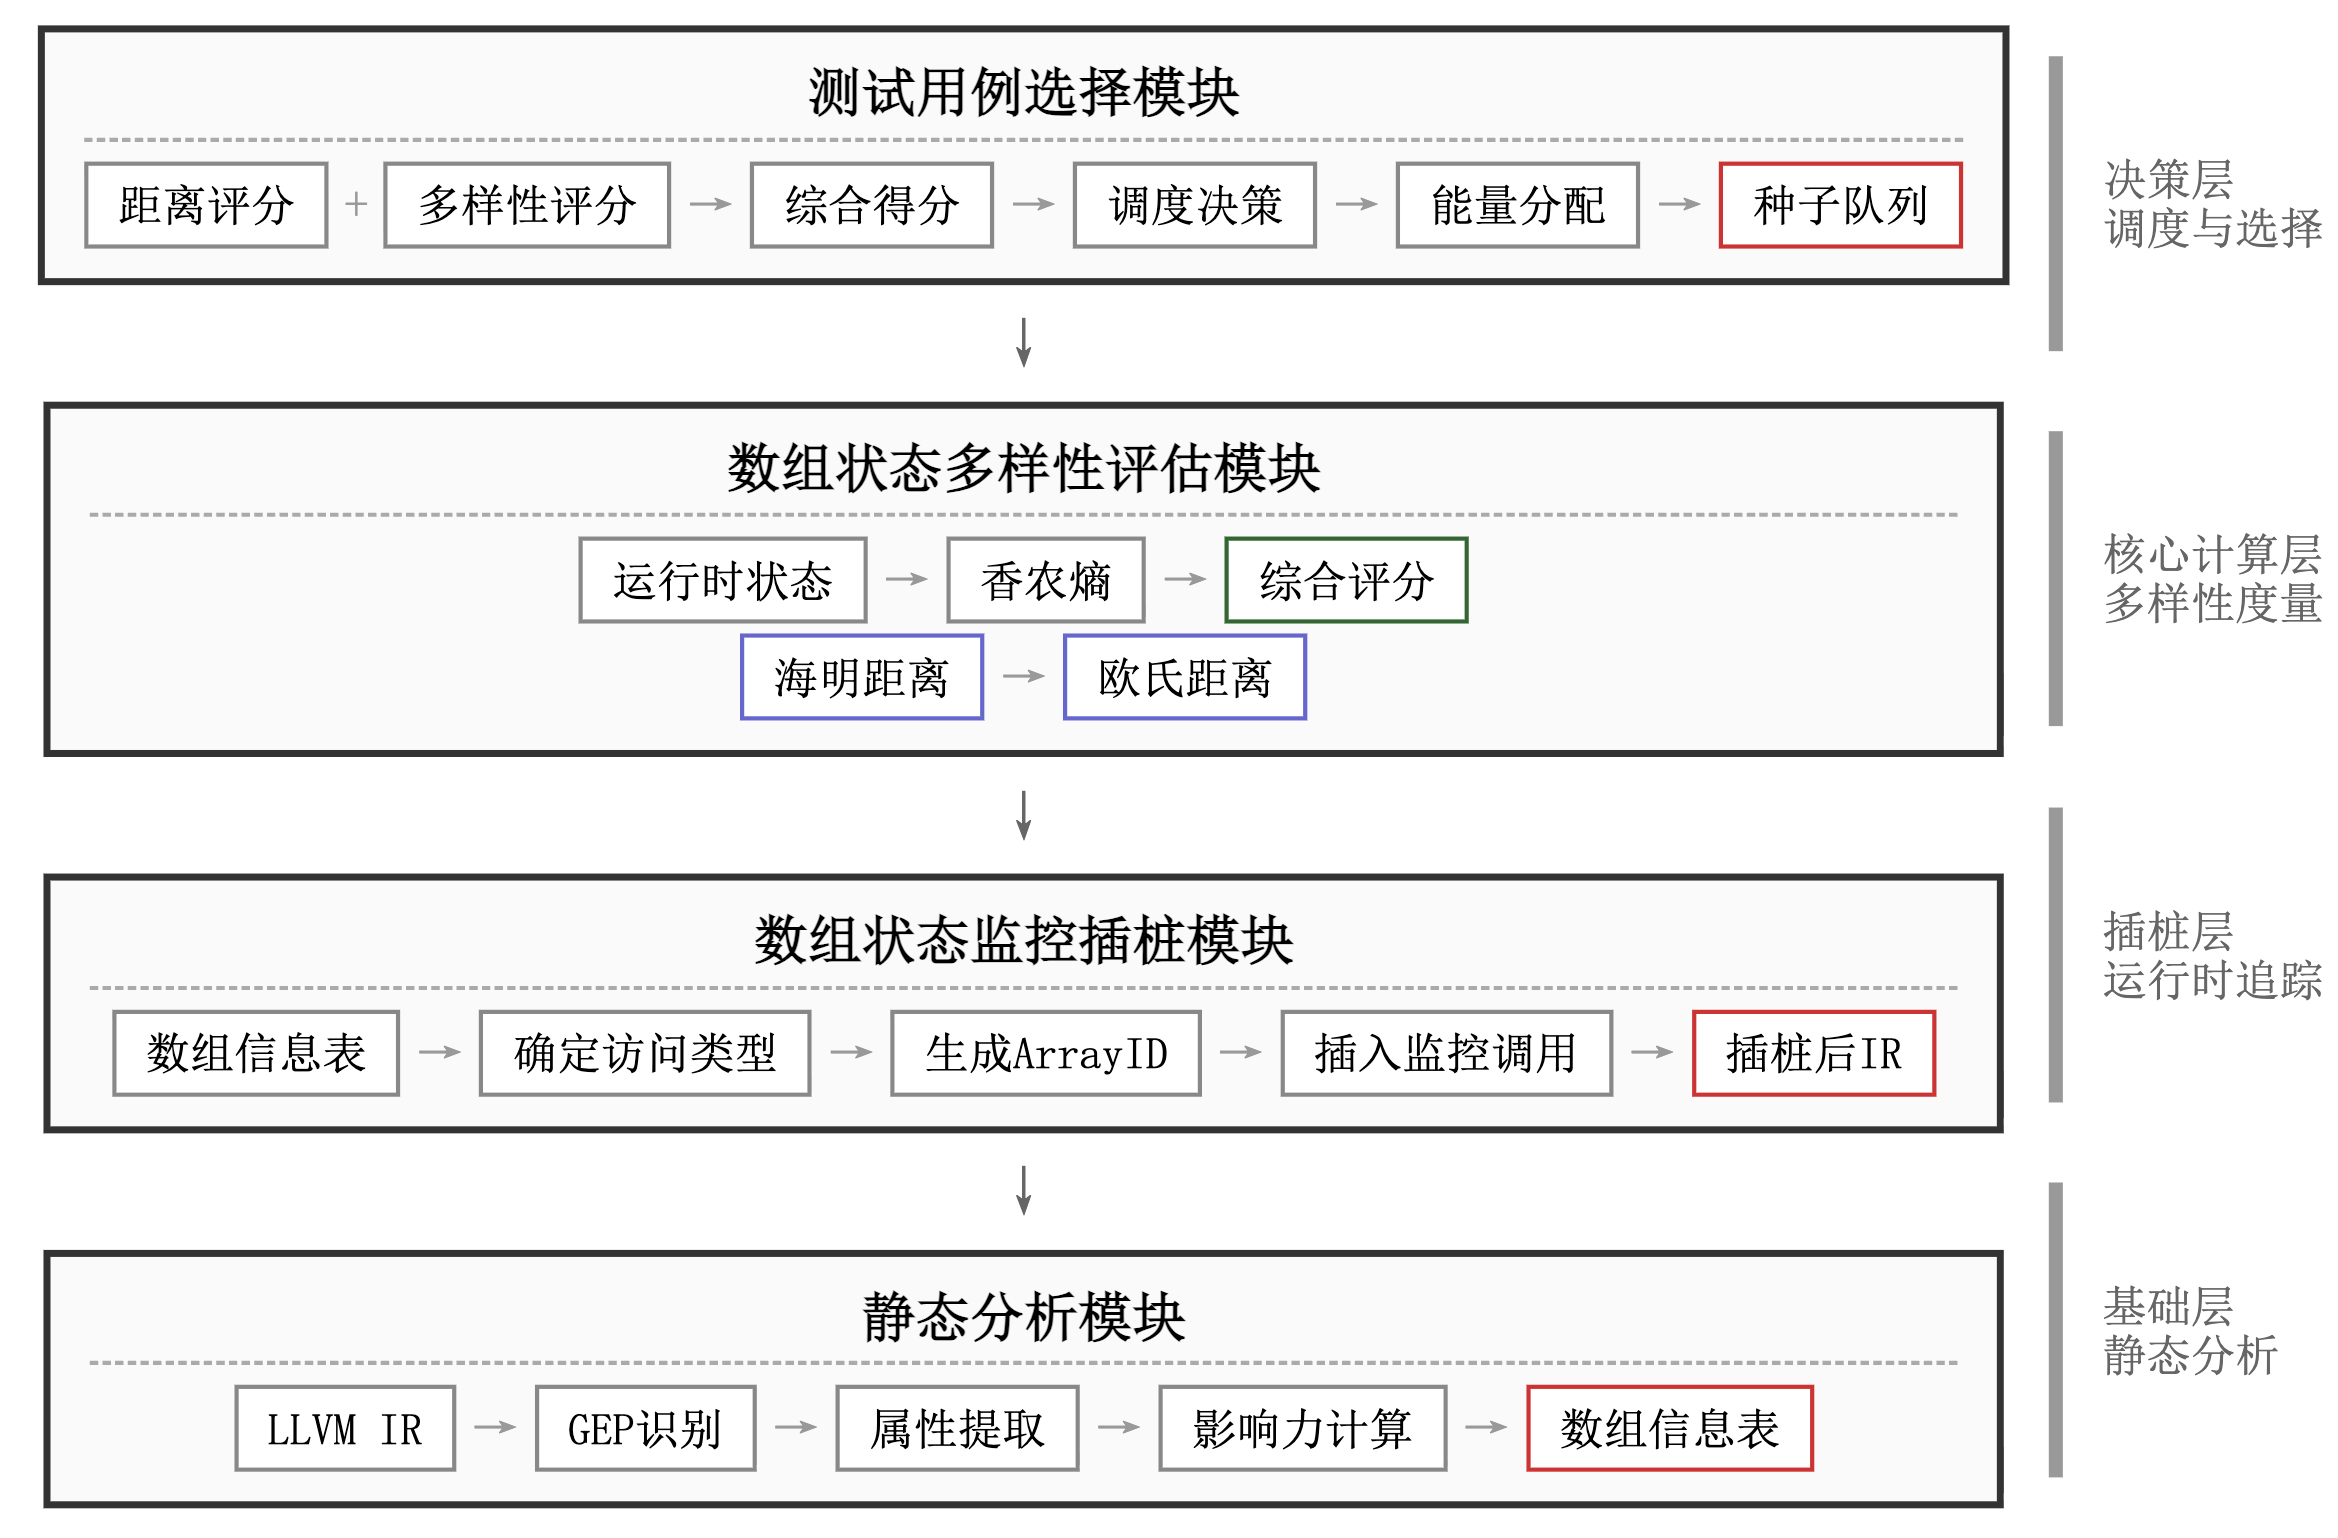
\includegraphics[width=0.85\textwidth]{figures/fig3_1_architecture.png}
\caption{系统总体架构图}
\label{fig:system_arch}
\end{figure}

系统各模块的职责和协作关系如下：

\textbf{（1）静态分析模块}位于系统架构的最底层，是其他模块的数据基础。该模块以目标程序的LLVM IR为输入，通过遍历和分析GEP指令，识别数组变量并提取相关属性信息，计算每个数组变量的影响力分数。分析结果以结构化的数组变量描述表的形式输出，同时供插桩模块和多样性评估模块使用。

\textbf{（2）数组状态监控插桩模块}接收静态分析模块输出的数组变量信息，在目标程序LLVM IR的GEP指令之后插入运行时监控函数的调用。该模块的插桩过程考虑了多维数组和不同访问类型的差异，为每个数组访问点生成包含数组ID、索引、访问类型和行号信息的监控调用。

\textbf{（3）数组状态多样性评估模块}在整个系统架构中处于核心计算位置。该模块通过运行时库接收插桩代码传递的状态信息，实时维护每个数组的访问记录。在执行过程中，该模块综合运用香农熵和状态多样性得分（SDS）两种度量方法计算多样性得分，并为测试用例选择模块提供量化评估结果。

\textbf{（4）测试用例选择模块}处于系统架构的决策层面。该模块接收多样性评估模块输出的评分结果和AFLGO框架的距离评分，通过综合得分函数计算每个测试用例的综合价值得分，并根据得分高低决定种子的调度优先级和变异能量的分配额度。

四个模块之间的数据流关系为：静态分析模块的输出是插桩模块的输入。插桩模块对目标程序进行改造后，在运行时产生数组状态数据。多样性评估模块对状态数据进行分析计算，产出评分结果。测试用例选择模块根据评分结果决定调度优先级，决策结果反馈到模糊测试的主循环中，形成一个完整的闭环反馈链路。

\subsection{系统工作流程}

系统的工作流程可以划分为三个阶段：准备阶段、执行阶段和分析阶段。

\textbf{准备阶段：}首先，用户提供目标程序的源代码路径和需要聚焦的目标代码位置（行号列表）。系统调用Clang编译器将目标程序源代码编译为LLVM IR中间表示。接着，静态分析模块对IR表示进行分析，识别数组变量并计算影响力分数，生成数组变量描述表。然后，插桩模块根据分析结果在数组访问位置插入监控代码。最后，经过插桩的IR被编译为可执行二进制文件，并与运行时库进行静态链接，生成可用于模糊测试的插桩版本目标程序。

\textbf{执行阶段：}系统启动模糊测试主循环。在每次迭代中，测试用例选择模块从种子队列中选取一个种子，运行插桩后的目标程序，同时启动运行时库进行状态追踪。执行完毕后，运行时库返回数组状态的多样性评分。测试用例选择模块将多样性评分与AFLGO的距离评分进行融合，计算综合得分，并将得分反馈给调度器。调度器根据综合得分决定该种子的变异能量（即为其生成的测试用例数量）。如果新生成的测试用例触发了新的代码路径或新的数组状态，则将其加入种子队列。

\textbf{分析阶段：}在测试执行过程中持续汇总测试中发现的程序崩溃和异常退出事件，按崩溃类型进行分类统计。同时记录覆盖率变化趋势，分析各数组变量的已探索槽位占比。最后将多样性评分的变化趋势与漏洞发现过程进行关联，验证多样性引导策略的实际效果。

\section{系统关键模块设计}

\subsection{静态分析模块}

静态分析模块借助LLVM Pass框架搭建，主要分析程序中的数组变量状态。它通过遍历函数的LLVM IR，识别GetElementPtr（GEP）指令中源元素类型为数组类型的指令，提取数组的名称、类型、长度、维度等属性信息。通过分析数组索引变量是否出现在条件分支的比较操作和循环结构的phi节点中，计算数组变量的影响力分数，量化其在程序控制流中的重要性。分析结果以数组变量描述表的形式输出，供后续的插桩模块和多样性评估模块使用。

\subsection{数组状态监控插桩模块}

数组状态监控插桩模块与静态分析结果紧密配合。在初始化阶段，模块读取静态分析输出的数组变量信息，建立数组ID到数组属性的映射表。在插桩阶段，模块遍历目标程序IR中的GEP指令，对每个源类型为数组类型的GEP指令依次处理。先通过分析GEP指令的use-def链确定访问类型（读或写），再通过函数名和变量名使用FNV-1a哈希算法生成数组的唯一标识ID。同时从GEP的操作数中提取索引值表达式，通过调试信息获取访问发生的源代码行号。然后在GEP指令之后插入对运行时报告函数\texttt{\_\_afl\_report\_array\_state}的调用，并将上述信息作为参数传递。

\subsection{数组状态多样性评估模块}

数组状态多样性评估模块通过监测程序运行时数组状态的变化，从两个维度综合评估数组状态探索程度：

（1）基于香农熵的分布均匀性度量：评估数组索引在不同槽位上的分布是否均匀，熵值越高说明探索了更多不同的索引位置，越有可能覆盖数组边界。

（2）基于状态多样性得分（SDS）的探索广度度量：通过统计已访问的索引槽位数与总槽位数的比例，衡量每个数组状态空间的覆盖程度。SDS越高说明数组的不同索引位置被探索得越充分。

两个指标相互补充，共同构成对数组状态探索程度的综合评价。

\subsection{测试用例选择模块}

测试用例选择模块将数组状态多样性评分与AFLGO原有的距离评分结合起来，设计综合得分函数。综合得分包含三个组成部分。距离评分反映测试用例执行路径到目标位置的接近程度，由AFLGO的距离计算引擎提供。多样性评分（SDS）反映测试用例触发的数组状态的探索广度，由多样性评估模块计算。香农熵评分反映数组索引访问分布的均匀程度，用于细化对数组访问模式的评估。通过加权融合，使测试资源更有效地分配到具有较高探索价值的测试用例上。

\section{本章小结}

本章完成了系统需求分析和概要设计。需求分析方面明确了工具需要满足的四项功能性需求（静态分析、插桩监控、多样性评估、测试用例选择）和四项非功能性需求（性能、可靠性、可扩展性、兼容性）。概要设计方面将系统划分为四个核心模块，阐述了各模块的职责划分、数据交互关系和工作流程。


% ======================================================================
% 第四章 系统详细设计与实现
% ======================================================================
\chapter{系统详细设计与实现}

\section{静态分析模块设计与实现}

静态分析模块是工具的基础环节，主要分析目标程序的LLVM IR中间表示，提取数组变量信息，为后续插桩、评估和测试用例生成提供数据支撑。该模块实现了两类核心操作：数组变量的精准识别和变量影响力的量化评估，其类结构如图~\ref{fig:class_static}所示。\\

\begin{figure}[hbt]
\centering
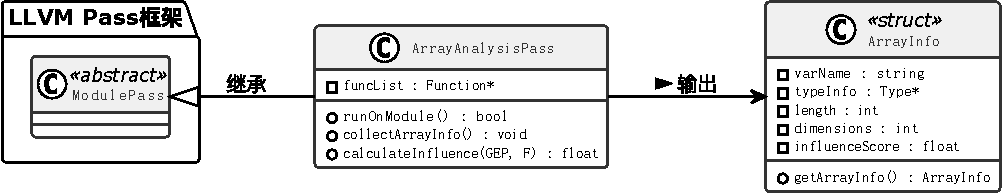
\includegraphics[width=0.85\textwidth]{figures/fig4_1_static_analysis_class}
\caption{静态分析模块类图}
\label{fig:class_static}
\end{figure}

图中\texttt{ArrayAnalysisPass}是LLVM Pass的主类，继承自\texttt{ModulePass}，通过重写\texttt{runOnModule}方法遍历模块中的所有函数和GEP指令。\texttt{ArrayInfo}结构体用于存储识别出的数组变量的各项属性信息，包括变量名、类型、长度、维度和影响力分数。数组变量识别逻辑和影响力计算算法分别通过\texttt{collectArrayInfo}和\texttt{calculateInfluence}两个内部方法实现。

\subsection{数组变量识别机制}

为了准确识别程序中的数组变量，本文设计了基于LLVM IR中GEP指令的数组分析算法。GEP（GetElementPtr）指令是LLVM IR中用于计算内存地址的关键指令，其语义天然暴露了数组的访问模式。对于数组类型变量，GEP指令的格式如下：

\begin{verbatim}
%ptr = getelementptr [10 x float], ptr %array, i64 0, i64 %idx
\end{verbatim}

该指令表示以\texttt{\%array}为基地址，经过两层偏移计算得到目标元素的指针。GEP指令的源元素类型为数组类型（\texttt{SourceTy->isArrayTy()}）时，即对应数组访问操作。

静态分析模块遍历目标程序的每个函数，扫描其中的GEP指令，对每个匹配的指令提取以下属性：数组名称（从指针操作数的符号名称提取）、类型信息（从源元素类型提取）、数组长度、维度信息（通过追溯嵌套GEP链确定）、作用域类型（全局变量、函数参数或栈上分配）。

\subsection{变量影响力计算}

为了评估数组变量在程序中的重要性，本文设计了变量影响力分析算法。该算法从以下维度计算每个数组变量的影响力分数：

\begin{itemize}
    \item 基础分为0.3，数组变量本身具有一定的重要性。
    \item 如果数组变量是函数参数，增加0.2分（参数传递的数组往往更关键）。
    \item 如果数组的索引值出现在条件分支的比较指令中，增加0.3分（条件表达式控制着程序的执行流向）。
    \item 如果数组的索引值在循环中通过phi节点更新，增加0.2分（循环控制变量影响多次迭代的访问）。
    \item 如果GEP指令被存储指令使用，增加0.1分（写操作影响数组内容）。
\end{itemize}

最终分数被归一化到$[0, 1]$区间。影响力分数越高的数组变量，在后续的多样性评估中被赋予更高的关注度。

\begin{table}[hbt]
\centering
\caption{数组变量影响力分析算法}
\label{tab:alg_influence}
\begin{tabular}{p{2.5cm} p{10cm}}
\toprule
\textbf{输入} & LLVM IR模块 \\
\midrule
\textbf{输出} & 数组变量信息表（名称、类型、长度、维度、影响力分数） \\
\midrule
\textbf{步骤} &
1. 遍历模块中的所有函数 \newline
2. 对每个函数，扫描所有GEP指令 \newline
3. 若GEP源类型为数组类型：\newline
\quad a. 提取数组名称、类型、长度、维度 \newline
\quad b. 通过use-def链追踪索引来源 \newline
\quad c. 判断索引是否出现在条件分支中 $\to$ 影响力加0.3 \newline
\quad d. 判断索引是否在循环phi节点中更新 $\to$ 影响力加0.2 \newline
\quad e. 判断GEP是否被存储指令使用 $\to$ 影响力加0.1 \newline
4. 归一化影响力分数至$[0,1]$区间 \newline
5. 输出结构化的数组信息表 \\
\bottomrule
\end{tabular}
\end{table}

核心实现代码如下所示：

\begin{verbatim}
float calculateInfluence(GetElementPtrInst *GEP, Function &F) {
    float score = 0.3f;  // 基础分
    Value *BasePtr = GEP->getPointerOperand();

    // 函数参数加分
    if (isa<Argument>(BasePtr)) score += 0.2f;

    // 分析索引来源是否与条件分支或循环相关
    Value *IdxVal = GEP->getOperand(GEP->getNumOperands() - 1);
    if (auto *Load = dyn_cast<LoadInst>(IdxVal)) {
        Value *Src = Load->getPointerOperand();
        for (auto &BB : F) {
            for (auto &Inst : BB) {
                if (auto *Br = dyn_cast<BranchInst>(&Inst)) {
                    if (Br->isConditional()) {
                        auto *ICmp = dyn_cast<ICmpInst>(Br->getCondition());
                        if (ICmp && (ICmp->getOperand(0) == Src ||
                                     ICmp->getOperand(1) == Src))
                            score += 0.3f;
                    }
                }
                if (isa<PHINode>(&Inst)) {
                    for (unsigned i = 0; i < Inst.getNumOperands(); i++)
                        if (Inst.getOperand(i) == Src) score += 0.2f;
                }
            }
        }
    }

    // 存储指令加分
    for (User *U : GEP->users())
        if (isa<StoreInst>(U)) { score += 0.1f; break; }

    return score > 1.0f ? 1.0f : score;
}
\end{verbatim}

静态分析模块的执行过程涉及多个组件之间的协作。图~\ref{fig:seq_static}以时序图的形式展示了静态分析模块的工作流程。

\begin{figure}[hbt]
\centering
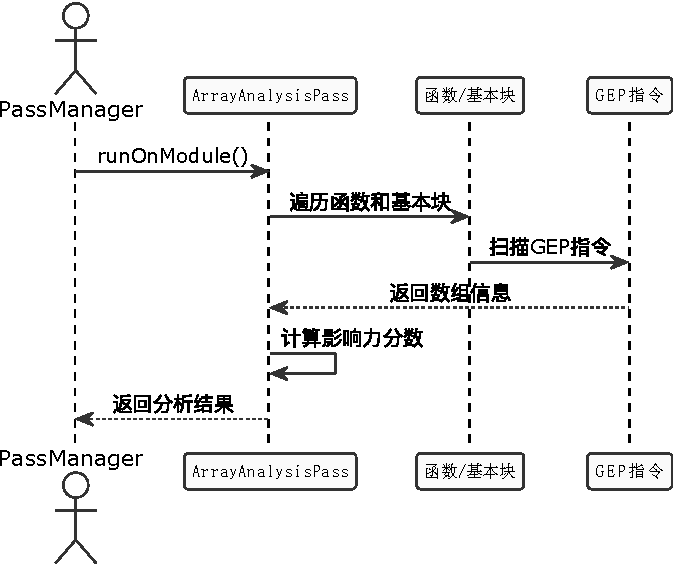
\includegraphics[width=0.85\textwidth]{figures/fig4_2_static_analysis_sequence}
\caption{静态分析模块时序图}
\label{fig:seq_static}
\end{figure}

该流程从\texttt{ArrayAnalysisPass}被Pass管理器调用开始，依次执行函数遍历、GEP指令识别、数组属性提取、影响力计算和结果输出等步骤，最终生成结构化的数组变量描述表供下游模块使用。

\section{数组状态监控插桩模块设计与实现}

数组状态监控插桩模块是工具中的关键组件，其主要功能是在数组访问的关键位置插入监控代码，收集数组的运行时状态信息。该模块基于LLVM Pass机制实现，通过分析和修改LLVM IR，在程序执行过程中对数组访问进行监控。该模块的类结构如图~\ref{fig:class_instr}所示。

\begin{figure}[hbt]
\centering
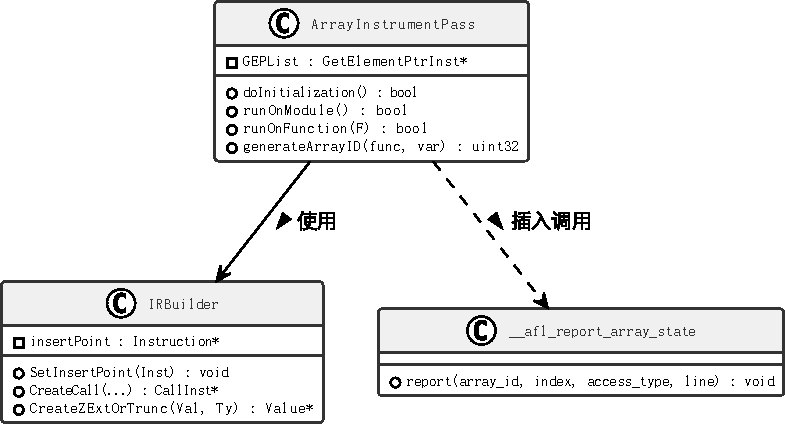
\includegraphics[width=0.85\textwidth]{figures/fig4_3_instrumentation_class}
\caption{数组状态监控插桩模块类图}
\label{fig:class_instr}
\end{figure}

\texttt{ArrayInstrumentPass}是LLVM Pass的主类，继承自\texttt{ModulePass}。它使用\texttt{IRBuilder}在GEP指令之后插入监控代码。数组ID由工具函数\texttt{generateArrayID}通过FNV-1a哈希算法生成，类型分析和维度信息提取在插桩过程中内联完成。

\subsection{插桩机制}

插桩模块在静态分析的基础上，通过IRBuilder在GEP指令之后插入对运行时报告函数\texttt{\_\_afl\_report\_array\_state}的调用。插桩的调用签名如下：

\begin{verbatim}
__afl_report_array_state(array_id, index, access_type, line_number)
\end{verbatim}

各参数的含义如下：\texttt{array\_id}（32位整数）为数组的唯一标识符，由函数名和变量名通过FNV-1a哈希生成。\texttt{index}（64位整数）为数组访问的索引值。\texttt{access\_type}（32位整数）为访问类型标志位，bit0表示读操作，bit1表示写操作。\texttt{line\_number}（32位整数）为访问发生的源代码行号。

插桩位置选择在GEP指令之后、内存访问指令（Load/Store）之前，确保采集到的索引值是该次访问的实际索引。对于多维数组，LLVM IR中会生成多个嵌套的GEP指令，每个维度对应一个GEP。模块对每个GEP分别插桩，并在生成ArrayID时对内层GEP追加"\#dimN"后缀，使不同维度的索引操作各自独立追踪。

\begin{table}[hbt]
\centering
\caption{数组访问监控插桩算法}
\label{tab:alg_instrument}
\begin{tabular}{p{2.5cm} p{10cm}}
\toprule
\textbf{输入} & 数组信息表、目标程序LLVM IR \\
\midrule
\textbf{输出} & 插桩后的LLVM IR \\
\midrule
\textbf{步骤} &
1. 读取数组信息表，建立ArrayID到数组属性的映射 \newline
2. 遍历目标程序IR中所有GEP指令 \newline
3. 对每个源类型为数组类型的GEP：\newline
\quad a. 通过use-def链确定访问类型（读/写） \newline
\quad b. 使用FNV-1a哈希生成ArrayID \newline
\quad c. 提取索引值表达式和源代码行号 \newline
\quad d. 在GEP后插入\texttt{\_\_afl\_report\_array\_state}调用 \newline
4. 处理多维数组：嵌套GEP分别插桩，内层添加\#dimN后缀 \newline
5. 输出插桩后的LLVM IR \\
\bottomrule
\end{tabular}
\end{table}

核心插桩代码如下所示：

\begin{verbatim}
// 对每个数组类型的GEP指令插桩
for (auto *GEP : targetGEPs) {
    // 确定访问类型（读/写）
    uint32_t accessType = 0;
    for (User *U : GEP->users()) {
        if (isa<LoadInst>(U)) accessType |= 1;
        else if (auto *SI = dyn_cast<StoreInst>(U))
            if (SI->getPointerOperand() == GEP) accessType |= 2;
    }
    if (accessType == 0) continue;

    // 获取行号
    uint32_t lineNum = 0;
    if (DILocation *Loc = GEP->getDebugLoc())
        lineNum = Loc->getLine();

    // 解析变量名和维度
    Value *BasePtr = GEP->getPointerOperand();
    std::string varName;
    int dimDepth = 0;
    Value *RootPtr = BasePtr;
    while (auto *InnerGEP = dyn_cast<GetElementPtrInst>(RootPtr)) {
        RootPtr = InnerGEP->getPointerOperand();
        dimDepth++;
    }
    varName = RootPtr->hasName() ? RootPtr->getName().str()
              : BasePtr->getName().str();

    // 多维数组维度区分
    if (dimDepth > 0)
        varName += "#dim" + std::to_string(dimDepth);
    uint32_t arrayID = generateArrayID(funcName, varName);

    // 提取索引值
    Value *RawIdx = GEP->getOperand(GEP->getNumOperands() - 1);
    if (!RawIdx->getType()->isIntegerTy()) continue;

    // 在GEP之后插入监控调用
    Builder.SetInsertPoint(GEP->getNextNode());
    Value *Idx64 = Builder.CreateZExtOrTrunc(RawIdx, Type::getInt64Ty(Ctx));
    Builder.CreateCall(ReportFunc, {
        Builder.getInt32(arrayID), Idx64,
        Builder.getInt32(accessType), Builder.getInt32(lineNum)
    });
}
\end{verbatim}

实际调试中发现，GEP指令嵌套在多个基本块之间时，插桩位置的选择会影响采集到的索引值的准确性，需要确保监控调用在索引值被修改之前执行。

图~\ref{fig:seq_instr}以时序图的形式展示了插桩模块将监控代码注入目标程序IR的过程。

\begin{figure}[hbt]
\centering
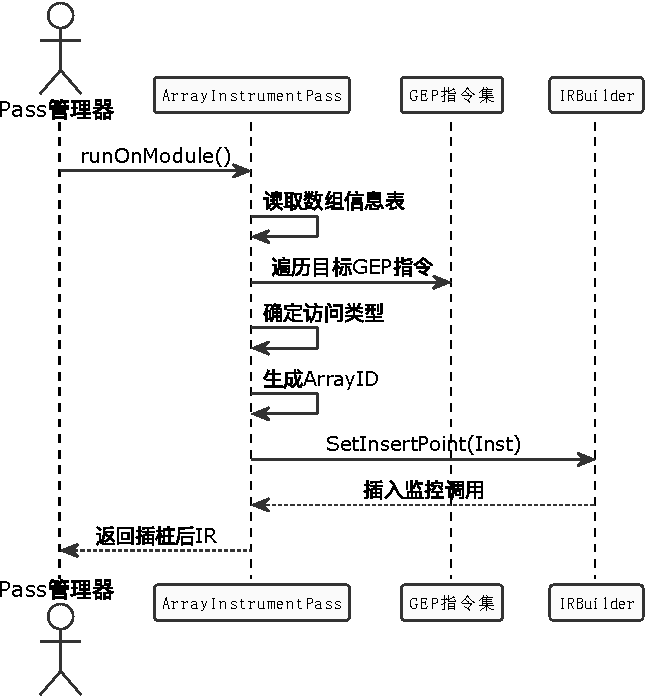
\includegraphics[width=0.85\textwidth]{figures/fig4_4_instrumentation_sequence}
\caption{数组状态监控插桩模块时序图}
\label{fig:seq_instr}
\end{figure}

在插桩过程中，模块依次完成读取分析结果、遍历GEP指令、确定访问类型、生成ArrayID和插入监控调用等步骤，最终输出经过插桩的LLVM IR文件。

\section{数组状态多样性评估模块设计与实现}

数组状态多样性评估模块是工具的核心组件之一，负责收集、分析和评估程序执行过程中数组变量的状态多样性。该模块通过插桩收集的运行时数据，综合运用多种度量方法评估数组状态空间的探索程度。该模块的类结构如图~\ref{fig:class_diversity}所示。

\begin{figure}[hbt]
\centering
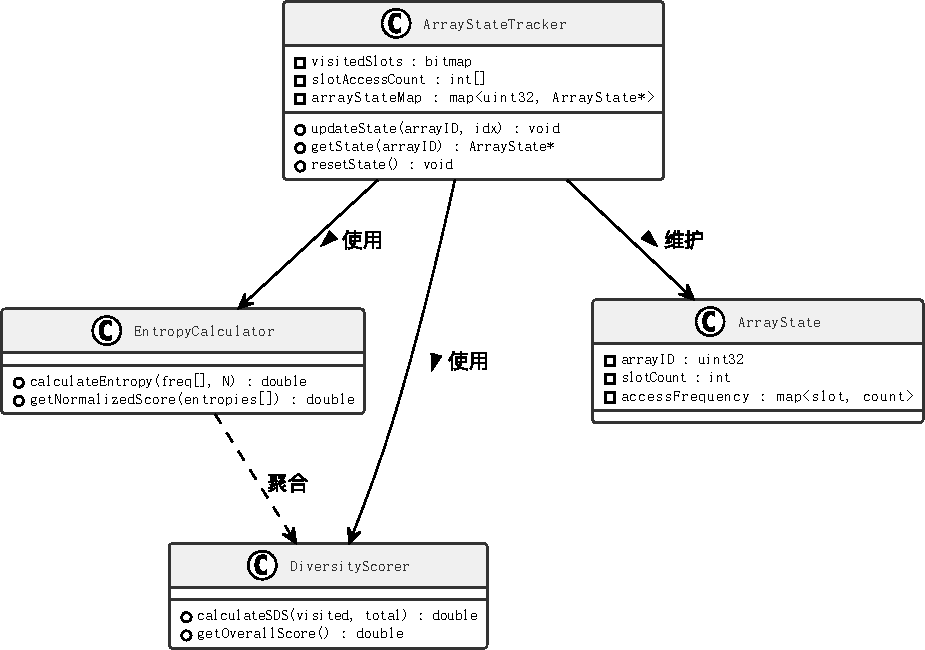
\includegraphics[width=0.85\textwidth]{figures/fig4_5_diversity_evaluation_class}
\caption{数组状态多样性评估模块类图}
\label{fig:class_diversity}
\end{figure}

\texttt{ArrayStateTracker}是核心的运行时状态追踪类，为每个数组维护一个\texttt{ArrayState}结构体，其中包含已访问的槽位位图（\texttt{visited\_slots}）和各槽位的访问频率数组（\texttt{slot\_access\_count}）。\texttt{EntropyCalculator}类实现香农熵的计算，\texttt{DiversityScorer}类实现状态多样性得分（SDS）的计算。

\subsection{基于香农熵的分布均匀性度量}

香农熵（Shannon Entropy）用于衡量数组索引访问在各槽位上的分布均匀程度。对于数组$a_i$，其访问熵定义为：

\begin{equation}
H_i = -\sum_{j=1}^{N} p_{ij} \log_2 p_{ij}
\end{equation}

其中$p_{ij} = c_{ij} / n_i$为槽位$j$被访问的频率（$c_{ij}$为槽位$j$的访问次数，$n_i$为总访问次数），$N$为总槽位数（本文设置为256）。当访问均匀分布时$H_i$达到最大值$\log_2 N$；当访问集中在少数槽位时$H_i$趋近于0。

全局归一化熵得分定义为：

\begin{equation}
E = \frac{1}{m} \sum_{i=1}^{m} \frac{H_i}{\log_2 N}
\label{eq:entropy_normalized}
\end{equation}

其中$m$为目标程序中已识别的数组变量总数。归一化后的$E \in [0, 1]$。

\begin{table}[hbt]
\centering
\caption{数组状态多样性评估算法}
\label{tab:alg_diversity}
\begin{tabular}{p{2.5cm} p{10cm}}
\toprule
\textbf{输入} & 插桩代码采集的运行时数组访问数据 \\
\midrule
\textbf{输出} & 香农熵得分$E$、状态多样性得分（SDS） \\
\midrule
\textbf{步骤} &
1. 初始化数组状态跟踪器，分配位图和频次数组 \newline
2. 接收插桩数据$(\text{arrayID}, \text{idx}, \text{type}, \text{line})$ \newline
3. 更新对应数组的访问位图和频次统计 \newline
4. 对每个数组$a_i$：\newline
\quad a. 计算各槽位访问频率$p_{ij} = c_{ij} / n_i$ \newline
\quad b. 计算香农熵$H_i = -\sum_j p_{ij} \log_2 p_{ij}$ \newline
\quad c. 计算SDS = 已访问槽位数 / 总槽位数 \newline
5. 计算全局归一化熵$E = \frac{1}{m}\sum_i H_i / \log_2 N$ \newline
6. 计算全局SDS = $\frac{1}{m}\sum_i \text{SDS}_i$ \newline
7. 输出$(E, \text{SDS})$至反馈文件 \\
\bottomrule
\end{tabular}
\end{table}

\section{测试用例选择模块设计与实现}

测试用例选择模块作为工具的核心调度组件，负责依据数组状态多样性和路径距离等多种因素，从测试用例队列中挑选出最具价值的测试用例进行变异和执行。该模块的类结构如图~\ref{fig:class_select}所示。

\begin{figure}[hbt]
\centering
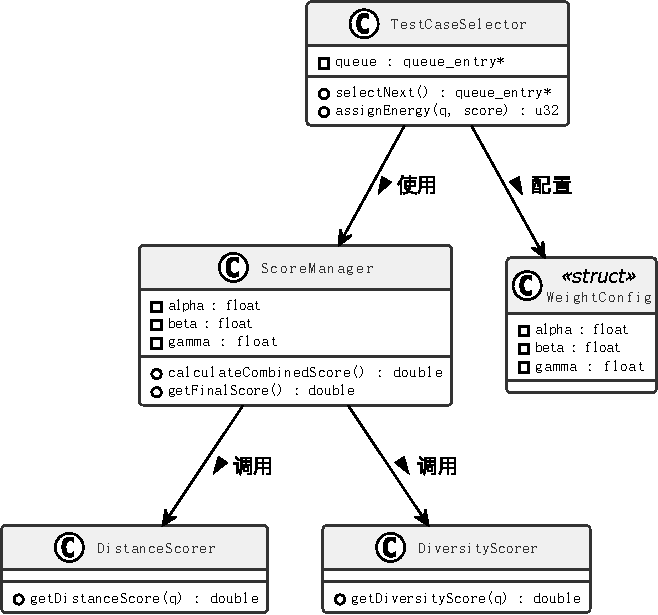
\includegraphics[width=0.85\textwidth]{figures/fig4_6_test_selection_class}
\caption{测试用例选择模块类图}
\label{fig:class_select}
\end{figure}

\texttt{ScoreManager}类负责综合评分的管理，它持有\texttt{DistanceScorer}和\texttt{DiversityScorer}两个评分子模块的引用，分别获取AFLGO距离评分和数组状态多样性评分。\texttt{WeightConfig}结构体封装了三个权重系数（$\alpha$、$\beta$、$\gamma$），可以通过配置文件进行调整。\texttt{TestCaseSelector}类根据综合得分进行调度决策，决定每个种子的变异能量和排队优先级。

\subsection{综合评分机制}

本文设计综合评分函数，将AFLGO原有的距离评分与数组状态多样性评估模块提供的两项指标，即状态多样性得分（SDS）和香农熵，融合为单一综合得分。距离评分反映了测试用例执行路径到目标位置的接近程度（距离越小越有价值）。SDS衡量测试用例覆盖的数组索引范围广度，香农熵衡量数组访问分布的均匀程度。

\begin{table}[hbt]
\centering
\caption{测试用例综合评分算法}
\label{tab:alg_scoring}
\begin{tabular}{p{2.5cm} p{10cm}}
\toprule
\textbf{输入} & 距离评分$D$、SDS评分$S$、香农熵$E$、权重系数$\alpha,\beta,\gamma$ \\
\midrule
\textbf{输出} & 综合得分$Q \in [0,1]$ \\
\midrule
\textbf{步骤} &
1. 距离评分转换：$D' = 1 / (D + 1)$，将距离映射到$[0,1]$ \newline
2. 计算综合得分：$Q = \alpha \cdot D' + \beta \cdot S + \gamma \cdot E$ \newline
3. 若handicap $\geq 4$：$Q = Q \times 4 / \text{handicap}$ \newline
4. 将$Q$截断至$[0,1]$范围 \newline
5. 返回$Q$作为种子的变异能量分配依据 \\
\bottomrule
\end{tabular}
\end{table}

综合得分函数的定义如下：

\begin{verbatim}
double calculate_combined_score(const score_input_t *input) {
    if (input->cal_failed) return 0.0;

    // 距离评分转换：距离越小越好，映射到 [0, 1]
    double dist_component = 1.0 / (input->distance_score + 1.0);

    // 综合得分 = alpha * dist + beta * SDS + gamma * entropy
    double score = weights.alpha * dist_component
                 + weights.beta  * input->diversity_score
                 + weights.gamma * input->entropy_score;

    // handicap 惩罚：handicap >= 4 时降权
    if (input->handicap >= 4)
        score *= 4.0 / (double)input->handicap;

    if (score < 0.0) score = 0.0;
    if (score > 1.0) score = 1.0;
    return score;
}
\end{verbatim}

其中权重系数$\alpha$、$\beta$、$\gamma$分别控制路径距离、数组状态多样性和访问分布均匀性在综合评分中的占比，默认设置为$\alpha=0.5$、$\beta=0.3$、$\gamma=0.2$。AFLGO原有的距离评分作为首要因子保留最高权重，确保工具的定向引导能力。SDS作为多样性探索的次要因子，香农熵作为分布均匀性的补充因子，用来细化对数组访问模式的评估。

综合得分策略在保留AFLGO定向能力的同时，引入数组状态多样性的探索引导，使模糊测试能在更短时间内、以更全面的方式探索数组的不同状态和路径。

图~\ref{fig:seq_overall}以时序图的形式展示了模糊测试过程中四个模块之间的协作关系。

\begin{figure}[hbt]
\centering
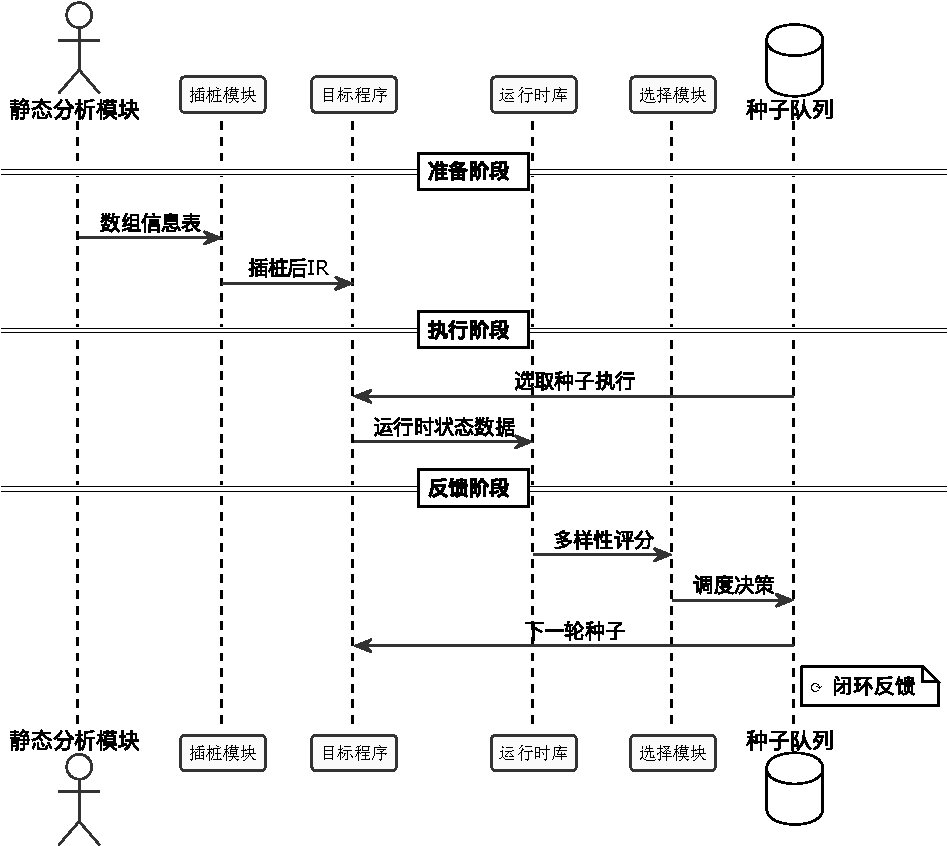
\includegraphics[width=0.85\textwidth]{figures/fig4_7_full_process_sequence}
\caption{模糊测试全过程模块协作时序图}
\label{fig:seq_overall}
\end{figure}

从时序图中可以看出，四个模块按照"静态分析→插桩→执行追踪→评分反馈→选择变异"的闭环流程协同工作。静态分析模块和插桩模块在测试准备阶段分析和改造目标程序，多样性评估模块和测试用例选择模块在测试执行阶段通过运行时反馈持续优化调度决策。

\section{本章小结}

本章完成了静态分析、数组状态监控插桩、数组状态多样性评估及测试用例选择四个核心模块的详细设计与实现。静态分析模块通过LLVM IR层面的GEP指令分析识别数组变量并计算影响力分数。数组状态监控插桩模块在GEP指令后插入监控代码，实现运行时数组状态的实时追踪。数组状态多样性评估模块使用香农熵和SDS两种方法量化状态差异。测试用例选择模块将评估结果与AFLGO距离评分融合，选出高价值测试用例。


% ======================================================================
% 第五章 系统测试
% ======================================================================
\chapter{系统测试}

本章在第三章需求分析与第四章详细设计的基础上，对系统各模块进行测试与评估。先介绍测试准备，包括测试环境和测试程序集。接着通过功能测试对系统功能进行验证。再通过对比实验评估工具相比AFLGO的有效性。

\section{测试准备}

\subsection{测试环境}

本次实验测试所选用的机器为 MacBook Air M3，搭载 Apple M3 处理器。机器配备 16GB 统一内存，运行 64 位 macOS 操作系统。实验环境依托Docker容器技术搭建，容器分配资源为 8GB 内存、60GB 存储空间、4 核 CPU，容器内部运行 Ubuntu 18.04.6 系统。开展对比实验所使用的工具为 AFLGO，版本号 2.57b。为避免其他运行因素干扰实验结果，所有环境配置、依赖部署及相关软件安装工作，均统一在同一 Docker 容器内完成，保障实验环境条件一致。

Docker容器基于Ubuntu 18.04基础镜像构建。首先安装LLVM 11工具链（包括clang-11、opt-11、llvm-link-11等）及其开发库。然后从AFLGO的官方仓库下载源代码并编译安装，使用LLVM Pass模式的afl-clang-fast编译器和相关的距离计算工具。再编译本文开发的数组分析Pass（array\_analysis\_pass.so）和数组插桩Pass（array\_instrument\_pass.so）。最后编译运行时库（libarray\_state.a），与LLVM Pass插件一同部署到容器的标准路径下。此外，所有被测程序均使用AddressSanitizer\cite{sanitizer}编译插桩，以便在测试过程中准确检测缓冲区溢出、越界访问等内存安全漏洞。

\subsection{测试程序集}

为了对AFLGO及本文工具进行测试，选取了AFLGO提供的开源测试程序集中较为典型的四个代码库进行实验，包括mjs、cjson、lrzip和libpng：

（1）mjs

mjs是为微控制器设计的轻量级JavaScript引擎，旨在实现ES6严格子集。它虽不提供标准库，但支持JSON.parse()和JSON.stringify()，并引入FFI用于直接调用C/C++函数。其特点是体积小巧，在32位ARM平台上占用资源少，且与C/C++兼容性佳。主要应用于嵌入式开发、物联网设备脚本运行等场景。

本次实验使用mjs的版本为d6c06a6，被测程序是mjs-bin，初始输入为空文件，运行参数为-f @@。

（2）cjson

cJSON是一个超轻量级的JSON解析器，使用C语言编写，具有代码量少、结构简单、解析效率高的特点。cJSON内部大量使用数组管理JSON对象、数组和嵌套结构，其JSON数组的解析过程涉及频繁的数组索引操作，数组访问模式的多样性直接影响代码路径的探索覆盖。在嵌入式系统和物联网应用的数据交换场景中被广泛使用。

本次实验使用cJSON的版本为v1.7.15，被测程序是cjson-bin，初始输入为小型JSON文件，运行参数为-f @@。

（3）lrzip

lrzip是一款大文件压缩工具，结合了rzip的预压缩能力和多种压缩算法（如LZMA、Bzip2、ZPAQ），能够高效处理海量数据。其主要特点是支持多线程压缩、解压速度较快、压缩比高，尤其适合处理包含大量冗余数据的大型文件，在数据备份和归档领域应用广泛。

本次实验使用lrzip的版本为9de7ccb，被测程序是lrzip，初始输入为小型文本压缩文件，运行参数为-t @@。

（4）libpng

libpng是PNG图像格式的官方参考库，支持PNG图像的创建、读取、写入等操作。在处理图像数据时，libpng频繁操作行缓冲区、像素数据等数组结构，大量数组访问分布在不同的图像解码路径中，数组状态的多样性对覆盖不同图像格式和处理选项有重要影响。在图像处理软件、游戏开发和Web浏览器等领域被广泛应用。

本次实验使用libpng的版本为1.6.37，被测程序是pngtest，初始输入为小型PNG图像文件，运行参数为-f @@。

测试程序集的具体配置信息如表5.1所示。准备这些测试程序时发现，部分代码库在版本更新后编译选项会发生变化，需要锁定具体commit来确保实验的可复现性。

\begin{table}[hbt]
\centering
\caption{测试程序集的配置信息}
\label{tab:targets}
\begin{tabular}{llll}
\toprule
\textbf{代码库} & \textbf{测试版本} & \textbf{被测程序} & \textbf{初始输入} \\
\midrule
mjs & d6c06a6 & mjs-bin & 空文件 \\
cjson & v1.7.15 & cjson-bin & JSON文件 \\
lrzip & 9de7ccb & lrzip & 小型文本压缩文件 \\
libpng & 1.6.37 & pngtest & PNG图像文件 \\
\bottomrule
\end{tabular}
\end{table}

\section{功能测试}

本节设计针对静态分析、数组状态监控插桩、数组状态多样性评估和测试用例选择四个功能模块的测试用例，并记录执行结果。

表5.2为静态分析的测试用例，验证模块能否准确识别程序中的数组变量。

\begin{table}[hbt]
\centering
\caption{静态分析测试用例}
\label{tab:tc1}
\begin{tabular}{ll}
\toprule
\textbf{项目} & \textbf{内容} \\
\midrule
用例ID & TC1 \\
用例名称 & 静态分析数组变量识别 \\
测试功能 & 验证静态分析模块能否准确识别程序中的数组变量 \\
测试步骤 & 1. 输入目标程序源代码 \\
& 2. 运行静态分析模块，生成数组变量列表及影响力评分 \\
预期结果 & 输出包含数组名称、类型、长度、影响力评分的结构化信息 \\
测试结果 & 与预期结果相符，成功识别目标程序中的所有数组变量 \\
\bottomrule
\end{tabular}
\end{table}

表5.3为数组状态监控插桩的测试用例，验证插桩模块能否在正确位置插入监控代码。

\begin{table}[hbt]
\centering
\caption{数组状态监控插桩测试用例}
\label{tab:tc2}
\begin{tabular}{ll}
\toprule
\textbf{项目} & \textbf{内容} \\
\midrule
用例ID & TC2 \\
用例名称 & 数组状态监控插桩 \\
测试功能 & 验证插桩模块能否在数组访问位置正确插入监控代码 \\
测试步骤 & 1. 导入静态分析生成的数组变量列表 \\
& 2. 对目标程序进行LLVM IR插桩 \\
& 3. 编译插桩后的程序，运行并监控数组访问记录 \\
预期结果 & 1. 插桩后程序正常编译运行 \\
& 2. 运行时正确记录数组ID、索引、类型和行号 \\
测试结果 & 与预期结果相符，运行时日志完整记录了所有数组访问事件 \\
\bottomrule
\end{tabular}
\end{table}

表5.4为数组状态多样性评估的测试用例，验证评估模块能否准确计算多样性指标。

\begin{table}[hbt]
\centering
\caption{数组状态多样性评估测试用例}
\label{tab:tc3}
\begin{tabular}{ll}
\toprule
\textbf{项目} & \textbf{内容} \\
\midrule
用例ID & TC3 \\
用例名称 & 数组状态多样性评估 \\
测试功能 & 验证评估模块能否准确计算多样性指标 \\
测试步骤 & 1. 运行插桩后的程序，输入测试用例 \\
& 2. 收集数组状态数据 \\
& 3. 检查香农熵、SDS等指标的计算结果 \\
预期结果 & 多样性指标随输入多样性增加而相应增长 \\
测试结果 & 与预期结果相符，SDS和熵值正确反映状态探索进展 \\
\bottomrule
\end{tabular}
\end{table}

表5.5为测试用例选择的测试用例，验证模块能否基于多样性评估结果选择测试用例。

\begin{table}[hbt]
\centering
\caption{测试用例选择测试用例}
\label{tab:tc4}
\begin{tabular}{ll}
\toprule
\textbf{项目} & \textbf{内容} \\
\midrule
用例ID & TC4 \\
用例名称 & 测试用例选择多样性引导 \\
测试功能 & 验证选择模块能否基于多样性评估结果选择测试用例 \\
测试步骤 & 1. 启用数组状态多样性引导模式 \\
& 2. 对目标程序进行模糊测试 \\
& 3. 对比常规模式与引导模式下的测试效果 \\
预期结果 & 引导模式下崩溃发现数量有所提升 \\
测试结果 & 与预期结果相符，引导模式提升了崩溃发现效率 \\
\bottomrule
\end{tabular}
\end{table}

\section{效果测试}

为了对本文设计并实现的模糊测试工具的实际效果进行评估，选取了4个程序代码库，分别用AFLGO和本文工具进行测试，统计路径发现数量、程序覆盖率和独特崩溃发现数量作为衡量指标，以综合评估测试工具的性能。

\subsection{评估指标}

（1）路径发现数量

路径发现数量衡量模糊测试系统发现全新执行路径的能力。该指标与代码覆盖率有关联，但更侧重于执行路径的多样性和新颖性。Böhme\cite{STADS}从物种发现的视角分析了软件测试中的多样性度量问题，为理解路径多样性与漏洞发现概率之间的关系提供了分析框架。模糊测试过程中，路径多样性直接决定了系统能否探索到程序的边缘状况，而这些边缘状况往往是安全漏洞频繁出现的区域。

本文提出的数组状态多样性引导通过监控数组索引状态的变化，有指向性地引导测试用例的生成，理论上可以更高效地探索程序的不同执行路径。测量路径发现数量可以直观评判该方法在引导测试用例生成上的有效性。

（2）程序覆盖率

程序覆盖率是评估模糊测试工具是否全面的关键指标，度量测试用例触及被测程序不同部分的范围广度。覆盖率越高，说明测试过程中执行了更多代码区域，发现潜在错误的可能性也越大。本文采用位图密度作为覆盖率的具体衡量方式，即被测程序中被覆盖的分支数量在整个位图中的占比。

本文方法关注数组状态的多样性，能生成更多样化的测试用例，理论上可以探索到更多程序执行路径。通过测量覆盖率的提升，可以评估该方法在拓展测试广度方面的效果，尤其针对那些不易触达的程序逻辑区域。

（3）独特崩溃发现数量

独特崩溃发现数量是模糊测试工具有效性最直观的体现，直接反映测试系统发现软件中潜在安全漏洞的能力。程序崩溃往往由空指针解引用、缓冲区溢出、整数溢出等问题引发，这些都属于严重的安全风险。

\subsection{实验结果与分析}

首先对测试过程中的路径发现数量进行统计与分析，以揭示本文提出的数组状态多样性引导的模糊测试方法的有效性。分别使用AFLGO与本文工具对测试程序集进行1h的对比测试，最终实验数据如表5.6所示：

\begin{table}[hbt]
\centering
\caption{路径发现数量统计}
\label{tab:paths}
\begin{tabular}{llll}
\toprule
\textbf{被测程序} & \textbf{测试工具} & \textbf{路径发现数量} & \textbf{增量} \\
\midrule
mjs & AFLGO & 2846 & \multirow{2}{*}{+116} \\
mjs & 本文工具 & 2962 & \\
\cmidrule(lr){2-4}
cjson & AFLGO & 935 & \multirow{2}{*}{+187} \\
cjson & 本文工具 & 1122 & \\
\cmidrule(lr){2-4}
lrzip & AFLGO & 1523 & \multirow{2}{*}{+85} \\
lrzip & 本文工具 & 1608 & \\
\cmidrule(lr){2-4}
libpng & AFLGO & 3524 & \multirow{2}{*}{+582} \\
libpng & 本文工具 & 4106 & \\
\bottomrule
\end{tabular}
\end{table}

整体来看，本文工具在4个被测代码库上的路径发现数量与AFLGO相比均有一定提升。其中cjson和libpng的提升最为显著，路径增量分别达到187条和582条，这得益于这两个库在JSON数组解析和图像行缓冲区处理中密集的数组访问操作，状态多样性引导能够更有效地探索数组边界附近的路径分支。mjs和lrzip的提升幅度相对较小，分别为116条和85条，这与它们的数组操作密度较低、状态空间有限的特性一致。

接着对测试过程中的程序覆盖率进行分析，以揭示使用本文改进策略后对模糊测试的性能提升。在一般情况下，更大的程序覆盖率意味着对被测程序的测试更加全面与充分，更有可能发现漏洞。实验数据如表5.7所示：

\begin{table}[hbt]
\centering
\caption{位图密度统计}
\label{tab:coverage}
\begin{tabular}{llll}
\toprule
\textbf{被测程序} & \textbf{测试工具} & \textbf{位图密度(\%)} & \textbf{增长率(\%)} \\
\midrule
mjs & AFLGO & 5.12 & \multirow{2}{*}{+0.12} \\
mjs & 本文工具 & 5.24 & \\
\cmidrule(lr){2-4}
cjson & AFLGO & 12.80 & \multirow{2}{*}{+1.92} \\
cjson & 本文工具 & 14.72 & \\
\cmidrule(lr){2-4}
lrzip & AFLGO & 6.78 & \multirow{2}{*}{+0.24} \\
lrzip & 本文工具 & 7.02 & \\
\cmidrule(lr){2-4}
libpng & AFLGO & 4.89 & \multirow{2}{*}{+0.64} \\
libpng & 本文工具 & 5.53 & \\
\bottomrule
\end{tabular}
\end{table}

在4个被测代码库上分别进行1h的测试后，与AFLGO相比，本文工具的位图密度均有一定增长。cjson的位图密度增长最为明显（+1.92个百分点），这是因为cjson代码规模较小且数组操作高度集中，状态引导在有限代码空间内产生了显著的覆盖扩散效果。libpng次之（+0.64个百分点），其图像解码路径中包含大量行缓冲区和像素数组访问，多样性引导有助于触及更多图像处理分支。mjs（+0.12个百分点）和lrzip（+0.24个百分点）的提升幅度较小，但同样表明数组状态多样性引导对程序覆盖率的提升有积极作用。

数组状态多样性引导机制可以探索到更深层次的程序分支，提升了发现独特崩溃的概率。实验数据如表5.8所示：

\begin{table}[hbt]
\centering
\caption{独特崩溃发现数量统计}
\label{tab:crashes}
\begin{tabular}{llll}
\toprule
\textbf{被测程序} & \textbf{测试工具} & \textbf{独特崩溃数量} & \textbf{增量} \\
\midrule
mjs & AFLGO & 2 & \multirow{2}{*}{+3} \\
mjs & 本文工具 & 5 & \\
\cmidrule(lr){2-4}
cjson & AFLGO & 3 & \multirow{2}{*}{+6} \\
cjson & 本文工具 & 9 & \\
\cmidrule(lr){2-4}
lrzip & AFLGO & 1 & \multirow{2}{*}{+2} \\
lrzip & 本文工具 & 3 & \\
\cmidrule(lr){2-4}
libpng & AFLGO & 2 & \multirow{2}{*}{+6} \\
libpng & 本文工具 & 8 & \\
\bottomrule
\end{tabular}
\end{table}

使用本文工具在4个被测代码库上分别进行1h的测试后，与AFLGO相比，独特崩溃发现数量均有一定增加。cjson和libpng的崩溃发现数量提升最大（分别增加6个），这两个库的数组越界和缓冲区溢出漏洞更容易通过数组状态引导被触发。lrzip新增2个崩溃，mjs新增3个，提升相对有限，这与它们的数组操作密度较低的情况相吻合。综合路径发现数量、程序覆盖率和独特崩溃发现数量三项指标来看，基于数组状态多样性的引导策略在mjs、cjson、lrzip和libpng这4个测试集上均有良好表现，相较于AFLGO有一定提升。

\section{本章小结}

本章完成了系统功能模块的测试和实验分析。首先明确了测试环境和测试程序集（mjs、cjson、lrzip、libpng）。接着设计了四个功能模块的测试用例，验证了系统功能。最后通过效果测试，从路径发现数量、程序覆盖率和独特崩溃发现数量三个维度评估了工具的有效性。实验表明，本文提出的数组状态多样性引导策略相比AFLGO取得了稳定提升。


% ======================================================================
% 结束语
% ======================================================================
\thesisconclusion

传统的模糊测试工具高度依赖代码覆盖率作为核心反馈指标，在探索程序内部变量的多样化状态时存在显著瓶颈。这类工具往往无法有效捕捉数组索引状态对漏洞触发的关键影响，在面对数组越界、缓冲区溢出等状态依赖型漏洞时，测试效率与漏洞发现能力较为低下。

本文设计并实现的数组状态多样性引导的模糊测试工具，通过四个核心模块的协同工作来提升测试效能。静态分析模块基于LLVM IR中间表示技术，通过GEP指令分析识别数组变量并量化其影响力。数组状态监控插桩模块在GEP指令后插入轻量级监控代码，实时追踪数组访问索引、类型和行号。数组状态多样性评估模块使用香农熵和状态多样性得分（SDS）两种方法，从分布均匀性和探索广度两个维度评估数组状态的探索程度。测试用例选择模块将状态多样性评分与AFLGO距离评分融合，优先变异高评分种子。在mjs、cjson、lrzip、libpng四个真实代码库的对比测试中，本文工具在路径发现数量、程序覆盖率和独特崩溃发现数量上均占优势。

本文的工作还存在以下不足和有待改进之处：

（1）测试对象数量有限。当前的测试针对4个开源代码库，虽然覆盖了不同类型的程序场景，但规模相对有限。未来需要在更多、规模更大的真实软件项目上进行更全面的评估。

（2）状态反馈与调度器的闭环集成不够紧密。当前状态多样性评分通过文件传递的方式供调度器使用，引入了一定的I/O开销。未来可以基于共享内存实现状态通信机制，实现零开销的实时反馈。

（3）数组类型覆盖不够全面。当前方法主要针对固定长度的栈上数组和全局数组进行插桩和追踪，对动态分配的堆数组的支持有限，未来可结合动态分析技术来获取缓冲区边界信息。

展望未来，本课题可以在以下方向进行深入研究和改进：一是将当前的数组状态追踪扩展为多维状态空间，全面建模数组、指针、结构体等多种变量的运行时状态。二是利用强化学习等技术，基于历史状态反馈数据自动学习最优的变异策略。三是在更多真实世界的大型软件项目中验证和改进本文方法。


% ======================================================================
% 致谢
% ======================================================================
\thesisacknowledgement
本论文的完成离不开王子元老师的悉心指导。从选题确定、方案设计到论文撰写，王老师始终给予我耐心的指导和宝贵的建议。王老师严谨的学术态度、渊博的专业知识以及对科研的执着追求，不仅指引我完成了这项研究，还对我未来的学术道路产生了深远影响。在此，谨向王老师致以最诚挚的感谢。

感谢计算机学院、软件学院、网络空间安全学院的各位老师在四年学习期间的谆谆教诲和无私帮助。正是老师们的辛勤耕耘，为我的专业学习和科研能力打下了坚实的基础。

感谢我的家人和朋友在求学期间给予我的理解、支持和鼓励。他们的支持是我不断前行的动力。

最后，感谢所有在模糊测试和软件安全领域做出贡献的研究者和开发者，他们的工作为本课题的研究提供了重要的基础和启示。

% ======================================================================
% 参考文献
% ======================================================================
\thesisreference

% ======================================================================
% 附录A 软件说明书
% ======================================================================
\thesisappendix

\section{引言}

本说明书为用户提供关于本文所设计并实现的数组状态多样性引导模糊测试工具的详细使用指南。通过阅读本说明书，用户能够了解该工具的基本原理、安装配置过程、具体使用方法以及测试结果分析等内容，能够高效、准确地运用该工具进行软件测试，发现潜在的安全漏洞和软件缺陷。

\section{工具概述}

\subsection{工具背景}

模糊测试作为一种重要的软件测试技术，通过向目标程序输入大量随机或半随机的数据，来发现程序中的漏洞和异常。传统的覆盖率引导模糊测试工具高度依赖代码覆盖率作为核心反馈指标，在探索程序内部数组变量状态方面存在显著瓶颈，难以高效触发数组越界、缓冲区溢出等状态依赖型漏洞。AFLGO是一种定向灰盒模糊测试工具，它在传统AFL的基础上引入了基于控制流图距离的定向引导机制，能够将测试资源聚焦于目标代码区域。本文工具在AFLGO的基础上，引入了数组状态多样性引导机制，通过追踪数组访问索引的运行时状态，从香农熵和状态多样性得分两个维度量化评估数组状态空间的探索程度，并将评估结果与AFLGO的距离评分相融合，形成双重引导体系。

\subsection{主要功能}

\textbf{数组变量静态分析}：基于LLVM Pass框架，自动扫描目标程序的LLVM IR中间表示，通过分析GetElementPtr（GEP）指令识别程序中的所有数组变量，并计算每个变量的影响力分数，为后续插桩点的选择提供参考。

\textbf{数组状态监控插桩}：在数组访问的GEP指令后自动插入轻量级运行时监控代码，在程序执行时实时采集数组唯一标识符、访问索引值、访问类型（读或写）以及源代码行号等信息。

\textbf{数组状态多样性评估}：运行时库维护每个数组的已访问槽位位图和频次统计，计算香农熵（衡量索引访问分布的均匀程度）和状态多样性得分SDS（衡量已探索索引槽位的广度），通过反馈文件将评估结果传递给模糊测试调度器。

\textbf{双引导融合调度}：将数组状态多样性评分（SDS和香农熵）与AFLGO原有的路径距离评分进行加权融合，形成综合得分Q。综合得分同时影响种子的变异能量分配和排队优先级，引导模糊测试更高效地探索数组状态空间中尚未覆盖的区域。

\subsection{工作原理}

本文工具在AFLGO的既有架构之上，引入了四个核心模块，形成了从静态分析、插桩、执行追踪、评分反馈到选择变异的闭环工作流程。

在测试准备阶段，静态分析模块对目标程序源代码进行LLVM IR层面的分析，识别所有数组变量并评估其影响力。插桩模块基于分析结果，在GEP指令后插入对运行时报告函数\texttt{\_\_afl\_report\_array\_state}的调用。

在测试执行阶段，每次运行目标程序时，插桩代码将数组访问信息传递给运行时库。运行时库实时更新各数组的访问位图和频次统计，并在程序退出时计算香农熵和SDS，写入反馈文件\texttt{/tmp/array\_feedback.txt}。

模糊测试器在校准阶段读取反馈文件中的SDS和熵值，调用综合得分函数\texttt{calculate\_combined\_score}计算融合得分Q。Q值影响该种子的变异能量（高Q获得更多变异循环次数）和排队优先级（高Q更容易被标记为favored，在队列中保持更活跃的变异频率）。通过这种机制，工具将数组状态多样性信息持续反馈到模糊测试的核心调度决策中。

\section{安装与配置}

\subsection{系统要求}

\begin{itemize}
\item \textbf{操作系统}：推荐使用Ubuntu 18.04及以上版本的Linux系统，支持通过Docker容器环境运行。
\item \textbf{编译器}：需要安装LLVM 11.0.0及相关的编译工具链（clang-11、opt-11、llvm-link-11等）。
\item \textbf{依赖库}：需要安装Python 3及相关Python库（如networkx、pydot等），用于AFLGO的距离计算脚本。
\item \textbf{Docker（可选）}：推荐使用Docker搭建统一的实验环境，避免依赖冲突。
\end{itemize}

\subsection{安装步骤}

\subsubsection{步骤1：克隆并编译AFLGO}

首先从AFLGO官方仓库克隆源代码，并编译AFLGO的核心组件：

\begin{verbatim}
git clone https://github.com/aflgo/aflgo.git /opt/aflgo
cd /opt/aflgo
make -C afl-2.57b
make -C instrument
make -C distance/distance_calculator
\end{verbatim}

\subsubsection{步骤2：编译LLVM Pass插件}

进入本文工具的Pass源码目录，使用CMake进行构建：

\begin{verbatim}
mkdir -p /workspace/passes/build && cd /workspace/passes/build
cmake .. -DLLVM_DIR=/usr/lib/llvm-11/cmake
make -j$(nproc)
\end{verbatim}

编译产物为\texttt{libarray\_analysis\_pass.so}（静态分析Pass）和\texttt{libarray\_instrument\_pass.so}（插桩Pass）。

\subsubsection{步骤3：编译运行时库}

进入运行时库目录，编译并打包为静态库：

\begin{verbatim}
cd /workspace/runtime
clang-11 -c -O2 -fPIC array_state_runtime.c -o array_state_runtime.o
ar rcs libarray_state.a array_state_runtime.o
\end{verbatim}

\subsubsection{步骤4：编译修改版AFLGo模糊器}

将本文提供的修改版配置文件和模糊器源码替换AFLGo原有文件后编译：

\begin{verbatim}
cd /opt/aflgo/afl-2.57b
cp /workspace/tmp-config.h config.h
cp /workspace/tmp-afl-fuzz.c afl-fuzz.c
AFL_NO_X86=1 make afl-fuzz
\end{verbatim}

\subsection{环境变量配置}

本文工具新增以下环境变量用于控制数组状态多样性引导功能：

\begin{itemize}
\item \textbf{AFL\_ARRAY\_DIVERSITY}：设置为1时启用数组状态多样性评估。程序退出时将SDS和熵值写入\texttt{/tmp/array\_feedback.txt}。
\item \textbf{AFL\_ARRAY\_FEEDBACK\_FILE}：指定反馈文件的自定义路径。若不设置，启用\texttt{AFL\_ARRAY\_DIVERSITY}后默认使用\texttt{/tmp/array\_feedback.txt}。
\end{itemize}

融合权重可通过修改\texttt{config.h}中的宏进行调整：

\begin{verbatim}
#define FUSION_WEIGHT_ALPHA  0.5   // 路径距离权重
#define FUSION_WEIGHT_BETA   0.3   // SDS多样性权重
#define FUSION_WEIGHT_GAMMA  0.2   // 香农熵权重
\end{verbatim}

\section{使用方法}

\subsection{准备目标程序}

首先获取目标程序的源代码并切换到指定的测试版本。以Git管理的项目为例：

\begin{verbatim}
git clone <目标程序仓库地址>
cd <目标程序目录>
git checkout <测试版本commit>
\end{verbatim}

\subsection{编译插桩后的目标程序}

本文工具提供两种编译模式。模式A为仅AFLGO边覆盖插桩（基线模式），模式B为AFLGO边覆盖加数组状态插桩（引导模式）。

\textbf{模式A（AFLGO基线）}：直接使用aflgo-clang编译：

\begin{verbatim}
/opt/aflgo/instrument/aflgo-clang -O0 -g <源文件> -o <输出文件> -lm
\end{verbatim}

\textbf{模式B（AFLGO + 数组状态引导）}：分步编译，先生成LLVM IR，叠加数组插桩Pass后再链接：

\begin{verbatim}
# 生成含AFLGo边覆盖的IR
/opt/aflgo/instrument/aflgo-clang -O0 -g -S -emit-llvm \
    <源文件> -o target.ll

# 叠加数组状态插桩
opt-11 -load /workspace/passes/build/libarray_instrument_pass.so \
    -array-instrument target.ll -S -o target_full.ll

# 编译并链接运行时库
clang-11 -O0 target_full.ll \
    /workspace/runtime/libarray_state.a \
    /opt/aflgo/instrument/aflgo-runtime.o \
    -o target_instr -lm
\end{verbatim}

对于多文件项目，需要先编译每个源文件为LLVM IR，再使用\texttt{llvm-link}合并所有IR文件，然后运行插桩Pass和最终链接。

\subsection{运行静态分析（可选）}

在编译前或编译后，可以单独运行静态分析Pass查看目标程序中数组变量的识别结果：

\begin{verbatim}
opt-11 -load /workspace/passes/build/libarray_analysis_pass.so \
    -array-analysis target.ll -o /dev/null 2> analysis_report.log
\end{verbatim}

分析报告包含每个函数中发现的数组变量名称、类型、长度、作用域和影响力评分。

\subsection{准备种子输入}

创建包含初始测试输入的种子目录。种子应为目标程序的有效输入。AFLGO会在这些种子的基础上进行变异，生成新的测试用例：

\begin{verbatim}
mkdir -p seeds
echo "<有效输入1>" > seeds/seed1.txt
echo "<有效输入2>" > seeds/seed2.txt
\end{verbatim}

\subsection{执行模糊测试}

使用编译好的afl-fuzz启动测试。模式B需要额外设置\texttt{AFL\_ARRAY\_DIVERSITY=1}：

\begin{verbatim}
# 模式A（基线）
AFL_NO_UI=1 AFL_SKIP_CPUFREQ=1 \
    /opt/aflgo/afl-2.57b/afl-fuzz \
    -i seeds -o output_A \
    -- ./target_A @@

# 模式B（数组状态多样性引导）
AFL_NO_UI=1 AFL_SKIP_CPUFREQ=1 \
AFL_ARRAY_DIVERSITY=1 \
    /opt/aflgo/afl-2.57b/afl-fuzz \
    -i seeds -o output_B \
    -- ./target_B @@
\end{verbatim}

其中\texttt{@@}为AFLGO的占位符，将被替换为实际的输入文件路径。

\section{测试结果分析}

剖析测试结果对于评估工具性能和发现潜在问题至关重要。AFLGO在测试进程中会生成详尽的统计信息，存储在输出目录的\texttt{fuzzer\_stats}文件中，包含以下关键指标：

\begin{itemize}
\item \textbf{execs\_done}：模糊测试执行的总测试用例数量。
\item \textbf{paths\_total}：测试过程中发现的独特执行路径总数，反映工具的路径探索能力。
\item \textbf{bitmap\_cvg}：位图覆盖率（百分比），表示被测程序中被覆盖的分支比例。
\item \textbf{unique\_crashes}：发现的独特崩溃数量，是工具漏洞发现能力最直接的体现。
\item \textbf{unique\_hangs}：发现的独特挂起数量，表示触发程序超时响应的测试用例数。
\item \textbf{cycles\_done}：完成的队列遍历轮数。
\item \textbf{pending\_total} / \textbf{pending\_favs}：队列中待处理的测试用例总数和favored用例数。
\end{itemize}

在模式B下，每次执行还会生成数组状态反馈文件\texttt{/tmp/array\_feedback.txt}，包含：

\begin{itemize}
\item \textbf{SDS}：状态多样性得分，反映数组索引槽位的整体探索比例。
\item \textbf{ENTROPY}：归一化香农熵得分，反映索引访问分布的均匀程度。
\item \textbf{NUM\_ARRAYS}：本次执行实际触发的数组数量。
\end{itemize}

通过对比模式A和模式B的上述指标，可以评估数组状态多样性引导机制对模糊测试性能的提升效果。

若在测试期间发现了崩溃，工具会将触发崩溃的测试用例保存在输出目录的\texttt{crashes/}子目录中。通过回放这些测试用例，可以复现和调试相关的漏洞。

\section{总结}

本文工具在AFLGO的基础上，引入了数组状态多样性引导机制，通过四个核心模块的协同工作提升模糊测试的效能。通过本说明书的介绍，用户可以了解工具的安装、配置和使用方法，以及测试结果的查看与分析步骤。在实际使用过程中，用户可以根据自己的需求和测试场景，灵活运用工具的各项功能，不断优化测试策略，提高测试质量。

\end{document}
